\documentclass[12pt, a4paper, english, singlespacing, parskip]{scrartcl}

%\documentclass[
%11pt, 				% The default document font size, options: 10pt, 11pt, 12pt
%oneside, 			% Two side (alternating margins) for binding by default, uncomment to switch to one side
%chapterinoneline,	% Have the chapter title next to the number in one single line
%english, 			% ngerman for German
%singlespacing, 	% Single line spacing, alternatives: onehalfspacing or doublespacing
%draft, 			% Uncomment to enable draft mode (no pictures, no links, overfull hboxes indicated)
%nolistspacing, 	% If the document is onehalfspacing or doublespacing, uncomment this to set spacing in lists to single
%liststotoc, 		% Uncomment to add the list of figures/tables/etc to the table of contents
%toctotoc, 			% Uncomment to add the main table of contents to the table of contents
%parskip, 			% Uncomment to add space between paragraphs
%nohyperref, 		% Uncomment to not load the hyperref package
%headsepline, 		% Uncomment to get a line under the header
%]{scrartcl or scrreprt or scrbook} % The class file specifying the document structure

\usepackage{amssymb, amsmath, color, graphicx, float, setspace, tipa}
\usepackage[utf8]{inputenc} 
\usepackage[english]{babel}
\usepackage[pdfpagelabels,pdfstartview = FitH,bookmarksopen = true,bookmarksnumbered = true,linkcolor = black,plainpages = false,hypertexnames = false,citecolor = black, breaklinks]{hyperref}
\usepackage{url}
\usepackage{caption}
\captionsetup{font=small,labelfont=bf, format=plain, justification=centering}
\allowdisplaybreaks 		% allows page breaks in align/equation environment

\usepackage{authblk} 		% titlepage stuff
\usepackage[titletoc, title]{appendix}



%--------------------------------------------
% NEW COMMANDS
%--------------------------------------------

\newcommand{\corresponds}{\mathrel{\widehat{=}}}		% equals with hat

\newcommand {\arctanh}{\mathrm{arctanh}}				% Atanh
\newcommand{\arccot}{\mathrm{arccot }}					% Acotanh

\newcommand{\limz}[1]{\lim\limits_{#1 \rightarrow 0}}	% Limes of something towars zero

\newcommand{\bm}{\boldmath}								% Bold font in math
\newcommand{\dps}{\displaystyle}						

\newcommand{\e}{\mbox{e}}								% e noncursive in math mode

\newcommand{\del}{\partial}								% partial diff operator
\newcommand{\de}{\mathrm{d}}							% differential d
\newcommand{\D}{\mathrm{d}}								% differential d
\newcommand{\GRAD}{\mathrm{grad}\ }						% gradient
\newcommand{\DIV}{\mathrm{div}\ }						% divergence
\newcommand{\ROT}{\mathrm{rot}\ }						% rotation

\newcommand{\CONST}{\mathrm{const.\ }}					% constant
\newcommand{\var}{\mathrm{var}}							% variance

\newcommand{\g}{^\circ}									% degrees
\newcommand{\degr}{^\circ}								% degrees

\newcommand{\msol}{M_\odot}								% solar mass


\newcommand{\x}{\mathbf{x}}								% x vector
\newcommand{\xdot}{\dot{\mathbf{x}}}					% x dot vector
\newcommand{\xddot}{\ddot{\mathbf{x}}}					% x doubledot vector
\newcommand{\R}{\mathbf{r}}								% r vector
\newcommand{\rdot}{\dot{\mathbf{r}}}					% r dot vector
\newcommand{\rddot}{\ddot{\mathbf{r}}}					% r doubledot vector
\newcommand{\vel}{\mathbf{v}}							% v vector
\newcommand{\V}{\mathbf{v}}								% v vector
\newcommand{\vdot}{\dot{\mathbf{v}}}					% v dot vector
\newcommand{\vddot}{\ddot{\mathbf{v}}}					% v doubledot vector

\newcommand{\dete}{\mathrm{d}t}							% dt
\newcommand{\delte}{\del t}								% partial t
\newcommand{\dex}{\mathrm{d}x}							% dx
\newcommand{\delx}{\del x}								% partial x
\newcommand{\der}{\mathrm{d}r}							% dr
\newcommand{\delr}{\del r}								% partial r

\newcommand{\deldt}{\frac{\del}{\del t}}				% shortcut partial derivative, in line
\newcommand{\ddt}{\frac{\de}{\de t}}					% shortcut total derivative, in line
\newcommand{\DELDT}[1]{\frac{\del  #1}{\del t}}			% shortcut partial derivative, on fraction
\newcommand{\DDT}[1]{\frac{\de  #1}{\de t}}				% shortcut total derivative, on fraction

\newcommand{\deldx}{\frac{\del}{\del x}}				% shortcut partial derivative, in line
\newcommand{\ddx}{\frac{\de}{\de x}}					% shortcut total derivative, in line
\newcommand{\DELDX}[1]{\frac{\del  #1}{\del x}}			% shortcut partial derivative, on fraction
\newcommand{\DDX}[1]{\frac{\de  #1}{\de x}}				% shortcut total derivative, on fraction

\newcommand{\deldr}{\frac{\del}{\del r}}				% shortcut partial derivative, in line
\newcommand{\ddr}{\frac{\de}{\de r}}					% shortcut total derivative, in line
\newcommand{\DELDR}[1]{\frac{\del  #1}{\del r}}			% shortcut partial derivative, on fraction
\newcommand{\DDR}[1]{\frac{\de  #1}{\de r}}				% shortcut total derivative, on fraction


\newcommand{\U}{\mathbf{U}}                             % state vector
\newcommand{\F}{\mathbf{F}}                             % flux tensor
\newcommand{\half}{\tfrac{1}{2}}

% quickly insert a figure without a caption
% usage: \quickfig{filename}{label}
\newcommand{\quickfig}[2]{
	\begin{figure}[H]
		\includegraphics[width=\textwidth]{#1}
		\caption{\label{#2}}
	\end{figure}
}


% replace \sum with \sum\limits
\let\oldsum\sum
\renewcommand{\sum}{\oldsum\limits}




%-----------------------------------------------
% FORMAT TITLE
%-----------------------------------------------


% Set fonts of document parts
\setkomafont{title}{\rmfamily\bfseries\boldmath}
\addtokomafont{section}{\rmfamily\bfseries\boldmath}
\addtokomafont{subsection}{\rmfamily\bfseries\boldmath}
\addtokomafont{subsubsection}{\rmfamily\bfseries\boldmath}
\addtokomafont{disposition}{\rmfamily} % table of contents and stuff
\setkomafont{descriptionlabel}{\rmfamily\bfseries\boldmath}

\usepackage{rotating}


%------------------------------------------
%: Metadata
%------------------------------------------

\title{Mesh Based Numerical Hydrodynamics of Ideal Gases}
\subtitle{The Used and Implemented Equations}
\author{Mladen Ivkovic (mladen.ivkovic@hotmail.com)}
\date{}

%------------------------------------------








\begin{document}
	
%--------------------------------------------
% Stuff that needs to be done before all else
%--------------------------------------------
%\pagestyle{plain}
%\nocite{*} % show all entries of bibliography, even if they are not cited.



%Titlepage
\maketitle
\newpage
\tableofcontents
\newpage



\newpage
%=======================================
\section{Ideal Gases}
%=======================================





%=======================================
\subsection{Governing Equations}
%=======================================

We are mostly going to concern ourselves with ideal gases, which are described by the Euler equations:


\begin{align}
	\deldt
	\begin{pmatrix}
		\rho \\
		\rho \V \\
		E
	\end{pmatrix}
	+
	\nabla \cdot
	\begin{pmatrix}
		\rho \V\\
		\rho \V \otimes \V + p\\
		(E + p) \V
	\end{pmatrix}
	=
	\begin{pmatrix}
		0\\
		\rho \mathbf{a}\\
		\rho \mathbf{a} \V
	\end{pmatrix}
\end{align}



Where
\begin{itemize}
	\item $\rho$: fluid density
	\item $\V$: fluid (mean/bulk) velocity at a given point. I use the notation $\V = (u, v, w)$, or when indices are useful, $\V = (v_1, v_2, v_3)$
	\item $p$: pressure
	\item $E$: specific energy. $E = \frac{1}{2} \rho \V^2 + \rho \varepsilon$, with $\varepsilon$ = specific internal thermal energy
	\item $\mathbf{a}$: acceleration due to some external force.
\end{itemize}

The outer product $\cdot \otimes \cdot$ gives the following tensor:
\begin{align}
	(\V \otimes \V)_{ij} = \V_i \V_j
\end{align}



Furthermore, we have the following relations for ideal gasses:
\begin{align}
	p &= n k T \\
	p &= C \rho ^ \gamma && \text{entropy relation for smooth flow, i.e. no shocks} \\
	s &= c_V \ln \left( \frac{p}{\rho^\gamma} \right) + s_0 && \text{entropy}\\
	a &= \sqrt{\frac{\del p}{\del \rho} \bigg{|}_s } = \sqrt{\frac{\gamma p}{\rho}} && \text{sound speed}
\end{align}

with 
\begin{itemize}
	\item $n$ : number density
	\item $k$ : Boltzmann constant
	\item $T$ : temperature
	\item $s$ : entropy
	\item $\gamma$: adiabatic index
	\item $c_V$: specific heat 
\end{itemize}

and the Equation of State

\begin{align}
	\varepsilon &= \frac{1}{\gamma - 1}\frac{p}{\rho}
\end{align}




The Euler equations can be written as a conservation law as

\begin{align}
    \DELDT{ \U } + \nabla \cdot \F(\U) = 0
\end{align}

where we neglect any outer forces, i.e. $\mathbf{a} = 0$, and 


\begin{align}
	\U = 
		\begin{pmatrix}
			\rho \\ \rho \V \\ E
		\end{pmatrix}, &&
	\F(\U) = 
		\begin{pmatrix}
			\rho \V\\
			\rho \V \otimes \V + p\\
			(E + p) \V
		\end{pmatrix}
\end{align}









%===============================================
\subsubsection{Euler equations in 1D}
%===============================================

In 1D, we can write the Euler equations without source terms ($\mathbf{a} = 0$) as 

\begin{align}
    \DELDT{ \U } + \DELDX{\F(\U)} = 0
\end{align}

or explicitly (remember $\V = (u, v, w)$)


\begin{align}
	\deldt{ 
		\begin{pmatrix}
			\rho \\ \rho u \\ E
		\end{pmatrix}
		}
	+ \deldx {
		\begin{pmatrix}
			\rho u\\
			\rho u^2  + p\\
			(E + p) u
		\end{pmatrix}
	} = 0
\end{align}




%===============================================
\subsubsection{Euler equations in 2D}
%===============================================

In 2D, we have without source terms ($\mathbf{a} = 0$)



\begin{align}
    \DELDT{ \U } + \DELDX{\F(\U)} + \frac{\del \mathbf{G}(\U)}{\del y} = 0
\end{align}

or explicitly  (remember $\V = (u, v, w)$)

\begin{align}
	\deldt{ 
		\begin{pmatrix}
			\rho \\ \rho u \\ \rho v \\ E
		\end{pmatrix}
		}
	+ \deldx {
		\begin{pmatrix}
			\rho u\\
			\rho u^2  + p\\
			\rho uv\\
			(E + p) u
		\end{pmatrix}
	} 
	+ \frac{\del}{\del y}
		\begin{pmatrix}
			\rho v\\
			\rho uv\\
			\rho v^2  + p\\
			(E + p) v
		\end{pmatrix}
	= 0
\end{align}















%===============================================
\subsection{Conserved and primitive variables}
%===============================================


For now, we have described the Euler equation as a hyperbolic conservation law using the (conserved) state vector $\U$:

\begin{align}
	\U = 
		\begin{pmatrix}
			\rho \\ \rho \V \\ E
		\end{pmatrix}
\end{align}


for this reason, the variables $\rho$, $\rho \V$, and $E$ are referred to as ``conserved variables'', as they obey conservation laws.

However, this is not the only set of variables that allows us to describe the fluid dynamics.
In particular, the solution of the  Riemann problem (section \ref{chap:riemann}) will give us a set of with so called ``primitive variables'' (or ``physical variables'') with the ``primitive'' state vector $\mathbf{W}$

\begin{align}
	\mathbf{W} = 
		\begin{pmatrix}
			\rho \\ \V \\ p
		\end{pmatrix}
\end{align}



Using the ideal gas equations, these are the equations to translate between primitive and conservative variables:

\textbf{Primitive to conservative:}

\begin{align}
	(\rho) &= (\rho) \\
	(\rho \V) &= (\rho) \cdot (\V) \\
	(E) &= \frac{1}{2} (\rho) (\V)^2 + \frac{1}{\gamma - 1} \frac{(p)}{(\rho)}
\end{align}


\textbf{Conservative to primitive:}

\begin{align}
	(\rho) &= (\rho) \\
	(\V) &= \frac{(\rho \V )}{(\rho)}\\
	(p) &= (\gamma - 1) \cdot (\rho)  \left((E) - \frac{1}{2} \frac{(\rho \V)^2}{(\rho)} \right) 
\end{align}













%=======================================
\subsection{Implementation Details}
%=======================================

All the functions for computing gas related quantities are written in \verb|gas.h| and \verb|gas.c|.
Every cell is represented by a struct \verb|struct cell| written in \verb|cell.h|.
It stores both the \underline{p}rimitive variables/states and the \underline{c}onservative states in the \texttt{\underline{p}state} and \texttt{\underline{c}state} structs, respectively.

The adiabatic index $\gamma$ is hardcoded as a macro in \texttt{defines.h}.
If you change it, all the derived quantities stored in macros (e.g. $\gamma - 1$, $\frac{1}{\gamma - 1}$) should be computed automatically.


\newpage
\section{Notation}


We are working on numerical methods.
Both space and time will be discretized.

Space will be discretized in cells which will have integer indices to describe their position.
Time will be discretized in fixed time steps, which may have variable lengths.
Nevertheless the time progresses step by step.

The lower left corner has indices $(0, 0)$ in 2D.
In 1D, index 0 also represents the leftmost cell.




We have:
\begin{itemize}
	\item integer subscript: Value of a quantity at the cell, i.e. the center of the cell. Example: $\U_i$, $\U_{i-2}$ or $\U_{i, j+1}$ for 2D.
	\item non-integer subscript: Value at the cell faces, e.g. $\F_{i-\half}$ is the flux at the interface between cell $i$ and $i-1$, i.e. the left cell as seen from cell $i$.
	\item integer superscript: Indication of the time step. E.g. $\U ^ n$: State at timestep $n$
	\item non-integer superscript: (Estimated) value of a quantity in between timesteps. E.g. $\F^{n + \half}$: The flux at the middle of the time between steps $n$ and $n + 1$.
\end{itemize}
\newpage


%====================================================================
\section{Riemann Problem and Solvers} \label{chap:riemann}
%====================================================================





%====================================================================
\subsection{The Riemann Problem and Solution Strategy}
%====================================================================




At the heart of Eulerian (not-comoving) numerical fluid dynamics is the solution to a specific initial value problem (IVP) called the ``Riemann problem''.
For a hyperbolic system of conservation laws of the form

\begin{align}
	\DELDT{\U} + \DELDX{\F(\U))} = 0
\end{align}

the Riemann problem is defined as

\begin{align}
	\U(x, t=0) = 
		\begin{cases}
			\U_L & \text{ if } x < 0\\
			\U_R & \text{ if } x > 0\\
		\end{cases}
\end{align}

see also fig. \ref{fig:riemann-problem}.

\begin{figure}[H]
	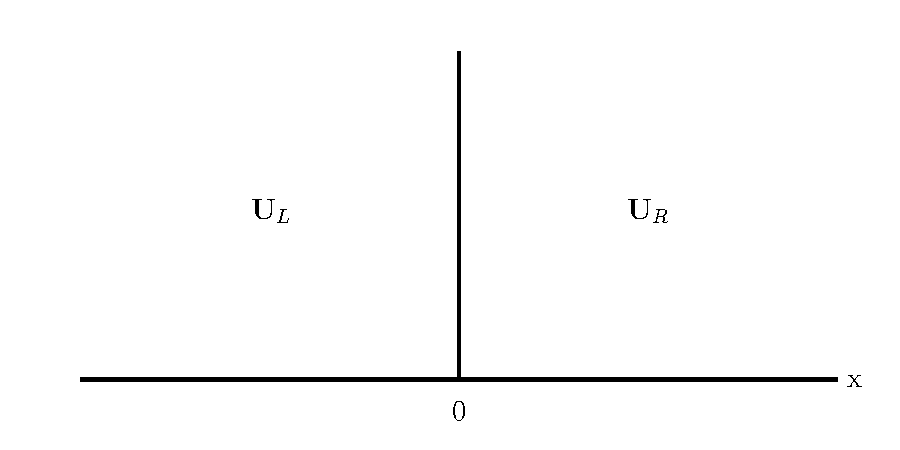
\includegraphics{./figures/riemann_problem.pdf}%
	\caption{
		The Riemann Initial Value Problem in 1D.
		\label{fig:riemann-problem}
	}
\end{figure}





Unfortunately, there is no exact closed-form solution to the Riemann problem for the Euler equations.
However, it is possible to devise iterative schemes whereby the solution can be computed numerically.
To solve full fluid dynamics problems, this calculation needs to be repeated many many times, making the solution quite expensive.
For that reason, people have developed approximate Riemann solvers, which we also will have a look at.



For a full derivation of how to solve the Riemann problem for the Euler equations, see e.g. \cite{toro}.
For our purposes, it suffices to accept that (assuming we have no vacuum) as time progresses, three waves will form which will separate the two initial states $\U_L$ and $\U_R$.
This results in two new states, $\U_L^*$ and $\U_R^*$ between the initial states, because  $\U_L^*$ and $\U_R^*$ themselves will be separated by a wave.
This is shown in figure \ref{fig:riemann-solution}


\begin{figure}[H]
	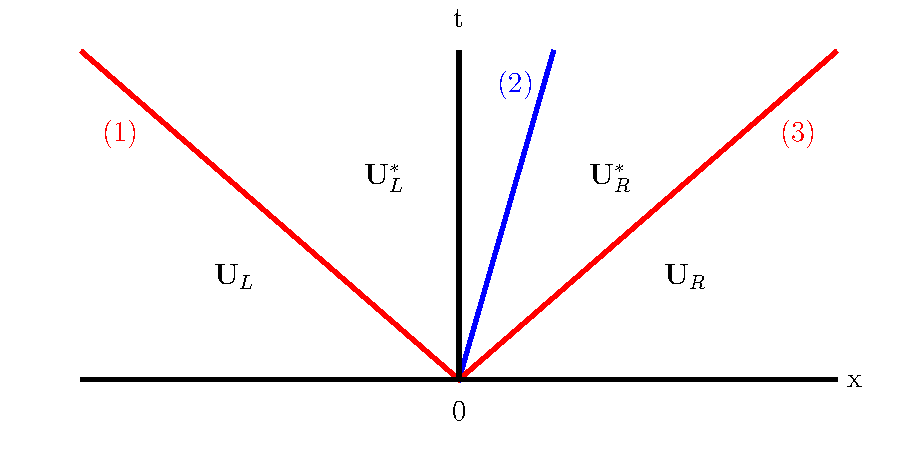
\includegraphics{./figures/riemann_solution.pdf}%
	\caption{
		The solution to the Riemann problem for Euler equations: 
		Three waves, (1), (2), and (3), arise from the origin as time evolves.
		(2) is always a contact wave, (1) and (3) can be either rarefaction or shock waves in each case, depending on the initial conditions.\\
		The initial states $\U_L$ and $\U_R$ are separated through the waves (1) and (3) from the two new arising ``star states'' $\U_L^*$ and $\U_R^*$, which themselves are separated by the contact wave (2).
		\label{fig:riemann-solution}
	}
\end{figure}












%===========================================
\subsection{Wave types and relations}
%===========================================





It turns out that we get three types of waves: A contact wave, a shock wave, and a rarefaction wave.
The middle wave is always a contact wave.
The left and right waves can be any combination of shock and/or rarefaction wave, depending on the initial conditions.
A model problem containing all three waves is shown in figure \ref{fig:riemann-solved}.
These are the wave properties:






%===========================================
\subsubsection{Contact wave}
%===========================================

The contact wave is a jump discontinuity in the density $\rho$ only.
Pressure and velocity remain constant across the contact wave.
This gives us the relations


\begin{align*}
	p^*_L &= p^*_R = p^*\\
	u^*_L &= u^*_R = u^*\\
\end{align*}

for this reason, the star state pressure and velocity will have no index indicating whether they are the left or right star state, and will be referred to as $p^*$ and $u^*$, respectively.









%===========================================
\subsubsection{Shock wave}
%===========================================

All three primitive variables $\rho$, $p$, and $u$ change across a shock wave.
A shock wave is a jump discontinuity too.
If the \textbf{leftmost} wave (wave (1) in fig. \ref{fig:riemann-solution}) is a shock wave, we have

\begin{align*}
	\rho^*_L &= 
		\frac{\frac{p^*}{p_L} + \frac{\gamma - 1}{\gamma+1}}{\frac{\gamma - 1}{\gamma+1} \frac{p^*}{p_L} + 1} \rho_L \\
	u^* &= 
		u_L - \frac{p^* - p_L}{\sqrt{\frac{p^* + B_L}{A_L}}}\\
		& = u_L - f_L(p^*) \\
	A_L &= 
		\frac{2}{(\gamma + 1) \rho_L}\\
	B_L &= 
		\frac{\gamma - 1}{\gamma + 1} p_L
\end{align*}

$f_{L}$ is given in eq. \ref{eq:riemann-pstar}, and the shock speed is
\begin{align*}
	S_L = u_L - a_L \left[\frac{\gamma + 1}{2 \gamma} \frac{p^*}{p_L} + \frac{\gamma - 1}{2\gamma} \right]^{\half}
\end{align*}

where $a_L$ is the sound speed in the left state $U_L$.



For a \textbf{right shock wave}, i.e. when wave (3) is a shock wave, we have the relations


\begin{align*}
	\rho^*_R &= 
		\frac{\frac{p^*}{p_R} + \frac{\gamma - 1}{\gamma+1}}{\frac{\gamma - 1}{\gamma+1} \frac{p^*}{p_R} + 1} \rho_R \\
	u^* &= 
		u_R + \frac{p^* - p_R}{\sqrt{\frac{p^* + B_R}{A_R}}}\\
		& = u_R + f_R(p^*) \\
	A_R &= 
		\frac{2}{(\gamma + 1) \rho_R}\\
	B_R &= 
		\frac{\gamma - 1}{\gamma + 1} p_R
\end{align*}

and the shock speed is
\begin{align*}
	S_R = u_R + a_R \left[\frac{\gamma + 1}{2 \gamma} \frac{p^*}{p_R} + \frac{\gamma - 1}{2\gamma} \right]^{\half}
\end{align*}

where $a_R$ is the sound speed in the left state $U_L$. $f_R$ is given in equation \ref{eq:riemann-pstar}.








%===========================================
\subsubsection{Rarefaction wave}
%===========================================

Rarefaction waves are smooth transitions, not infinitesimally thin jump discontinuities.
This makes them really easy to spot in the solutions of Riemann problems, see fig. \ref{fig:riemann-solved}.
Across rarefactions, entropy is conserved.

The rarefaction waves are enclosed by the head and the tail of the wave, between which we have a smooth transition which is called the ``fan''.
The head is the ``front'' of the wave, i.e. the part of the wave that gets furthest away from the origin as time progresses.
The tail is the ``back'' of the wave, i.e. the part of the wave that stays closest to the origin as time progresses.
The wave speeds of the head, $S_H$, and of the tail, $S_T$, are both given below.


If we have a \textbf{left-facing} rarefaction, i.e. if wave (1) is a rarefaction wave, we have

\begin{align*}
	\rho^*_L &= 
		\rho_L \left( \frac{p^*}{p_L} \right) ^ \frac{1}{\gamma}\\
	u^* &= 
		u_L - \frac{2 a_L}{\gamma - 1} \left[ \left( \frac{p^*}{p_L} \right) ^ \frac{\gamma - 1}{2 \gamma} -1  \right]\\
		& = u_L - f_L(p^*) \\
\end{align*}

$f_{L}$ is given in eq. \ref{eq:riemann-pstar}, and $a_L$ is the sound speed in the left state $U_L$.


The wave speeds of the head, $S_H$, and the tail, $S_T$, for the left facing wave are
\begin{align*}
	S_{HL} &= u_L - a_L\\
	S_{TL} &= u^* - a^*_L\\
	a^*_L  &= a_L \left( \frac{p^*}{p_L} \right) ^ \frac{\gamma - 1}{2 \gamma}
\end{align*}


Finally, the solution inside the rarefaction fan, i.e. in regions where $S_{HL} \leq \frac{x}{t} \leq S_{TL}$, is 

\begin{align*}
	\rho_{\text{fan}, L} &= 
		\rho_L \left[ \frac{2}{\gamma + 1} + \frac{\gamma - 1}{\gamma + 1} \frac{1}{a_L} \left(u_L - \frac{x}{t}\right) \right] ^ \frac{2}{\gamma -1 }\\
	u_{\text{fan}, L} &= 
		\frac{2}{\gamma + 1} \left[ \frac{\gamma - 1}{2} u_L + a_L + \frac{x}{t}  \right] \\
	p_{\text{fan}, L} &= 
		p_L \left[ \frac{2}{\gamma + 1} + \frac{\gamma - 1}{\gamma + 1} \frac{1}{a_L} \left(u_L - \frac{x}{t}\right) \right] ^ \frac{2 \gamma}{\gamma -1}
\end{align*}









If we have a \textbf{right-facing rarefaction}, i.e. if wave (1) is a rarefaction wave, we have

\begin{align*}
	\rho^*_R &= 
		\rho_R \left( \frac{p^*}{p_R} \right) ^ \frac{1}{\gamma}\\
	u^* &= 
		u_R - \frac{2 a_R}{\gamma - 1} \left[ 1 - \left( \frac{p^*}{p_R} \right) ^ \frac{\gamma - 1}{2 \gamma}  \right]\\
		&= u_R + f_R(p^*)
\end{align*}

where $a_R$ is the sound speed in the left state $U_R$.
$f_R$ is given in equation \ref{eq:riemann-pstar}.





The wave speeds of the head, $S_H$, and the tail, $S_T$, for the left facing wave are
\begin{align*}
	S_{HR} &= u_R + a_R\\
	S_{TR} &= u^* + a^*_R\\
	a^*_R  &= a_R \left( \frac{p^*}{p_R} \right) ^ \frac{\gamma - 1}{2 \gamma}
\end{align*}




Finally, the solution inside the rarefaction fan, i.e. in regions where $S_{HL} \leq \frac{x}{t} \leq S_{TL}$, is 

\begin{align*}
	\rho_{\text{fan}, R} &= 
		\rho_R \left[ \frac{2}{\gamma + 1} - \frac{\gamma - 1}{\gamma + 1} \frac{1}{a_R} \left(u_R - \frac{x}{t}\right) \right] ^ \frac{2}{\gamma -1 }\\
	u_{\text{fan}, R} &= 
		\frac{2}{\gamma + 1} \left[ \frac{\gamma - 1}{2} u_R - a_R + \frac{x}{t}  \right] \\
	p_{\text{fan}, R} &= 
		p_R \left[ \frac{2}{\gamma + 1} - \frac{\gamma - 1}{\gamma + 1} \frac{1}{a_R} \left(u_R - \frac{x}{t}\right) \right] ^ \frac{2 \gamma}{\gamma -1}
\end{align*}












%===========================================
\subsubsection{Which wave type do we have?}
%===========================================


As written before, the middle wave (wave (2) in fig. \ref{fig:riemann-solution} ) is always a contact wave, while the other two waves are any combination of rarefaction and/or shock wave.
It turns out that the condition for a rarefaction or shock wave is remarkably simple.

For the left wave (wave (1)):

\begin{align}
	p^* > p_L: && &\quad \text{ (1) is a shock wave}\\
	p^* \leq p_L: && &\quad \text{ (1) is a rarefaction wave}
\end{align}

and for the right wave (wave (3)):

\begin{align}
	p^* > p_R: && & \quad \text{ (3) is a shock wave} \\
	p^* \leq p_R: && & \quad \text{ (3) is a rarefaction wave} 
\end{align}

See \cite{toro} for more details.










%===========================================
\subsubsection{Solution for $p^*$}
%===========================================

The only thing missing to have a complete solution to the Riemann problem for the Euler equations is an expression how to obtain $p^*$, the pressure in the star region, depending on the initial conditions $U_L$ and $U_R$.
We make use of the fact that $p^*$ and $u^*$ are constant across the star region to relate $U_L$ and $U_R$, or more precisely the primitive states $\mathbf{W}_L$ and $\mathbf{W}_R$ which can easily be derived from the conservative ones.
For both shock and rarefaction waves on either side, we have equations for $u^*$ depending on the outer states  $\mathbf{W}_L$ and $\mathbf{W}_R$ and $p^*$.
By setting $u^*_L - u^*_R = 0$, which must hold, we get the equation

\begin{align}
	f(p, \mathbf{W}_L, \mathbf{W}_R) \equiv f_L(p, \mathbf{W}_L) + f_R(p, \mathbf{W}_R) + (u_R - u_L) = 0 \label{eq:riemann-pressure-equation}
\end{align}

with 

\begin{align}
	f_{L,R} &= 
		\begin{cases}
			(p - p_{L,R}) \left[ \frac{A_{L,R}}{p + B_{L,R}} \right]^{\frac{1}{2}}
				& ~\text{ if } ~ p > p_{L,R} ~ \quad \text{(shock)} \\
			\frac{2 a_{L,R}}{\gamma - 1} \left[ \left( \frac{p}{p_{L,R}} \right)^ \frac{\gamma -1}{2 \gamma} - 1 \right]
				& ~\text{ if } ~ p \leq p_{L,R} ~ \quad \text{(rarefaction)} \label{eq:riemann-pstar}\\
		\end{cases} \\
	A_{L,R} &= 
		\frac{2}{(\gamma + 1) \rho_{L,R}}\\
	B_{L,R} &= 
		\frac{\gamma - 1}{\gamma + 1} p_{L,R}
\end{align}












\begin{figure}
	\centering
	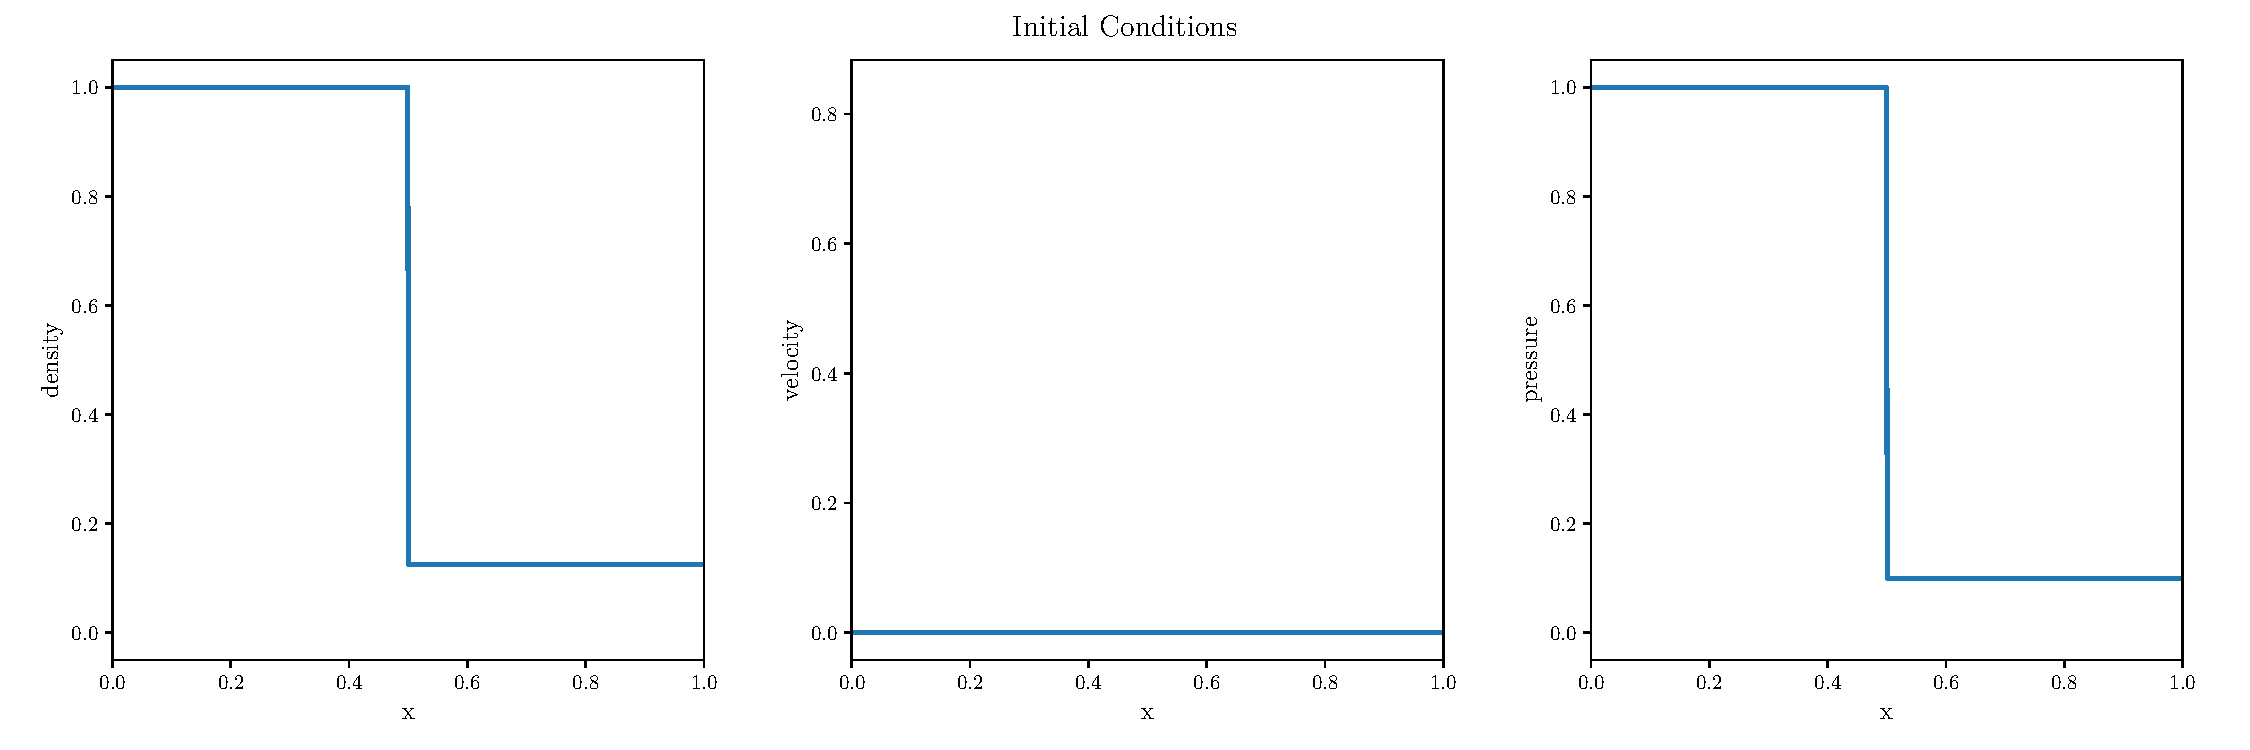
\includegraphics[width=.9\textwidth]{./figures/riemann_IC.pdf}%
	\\
	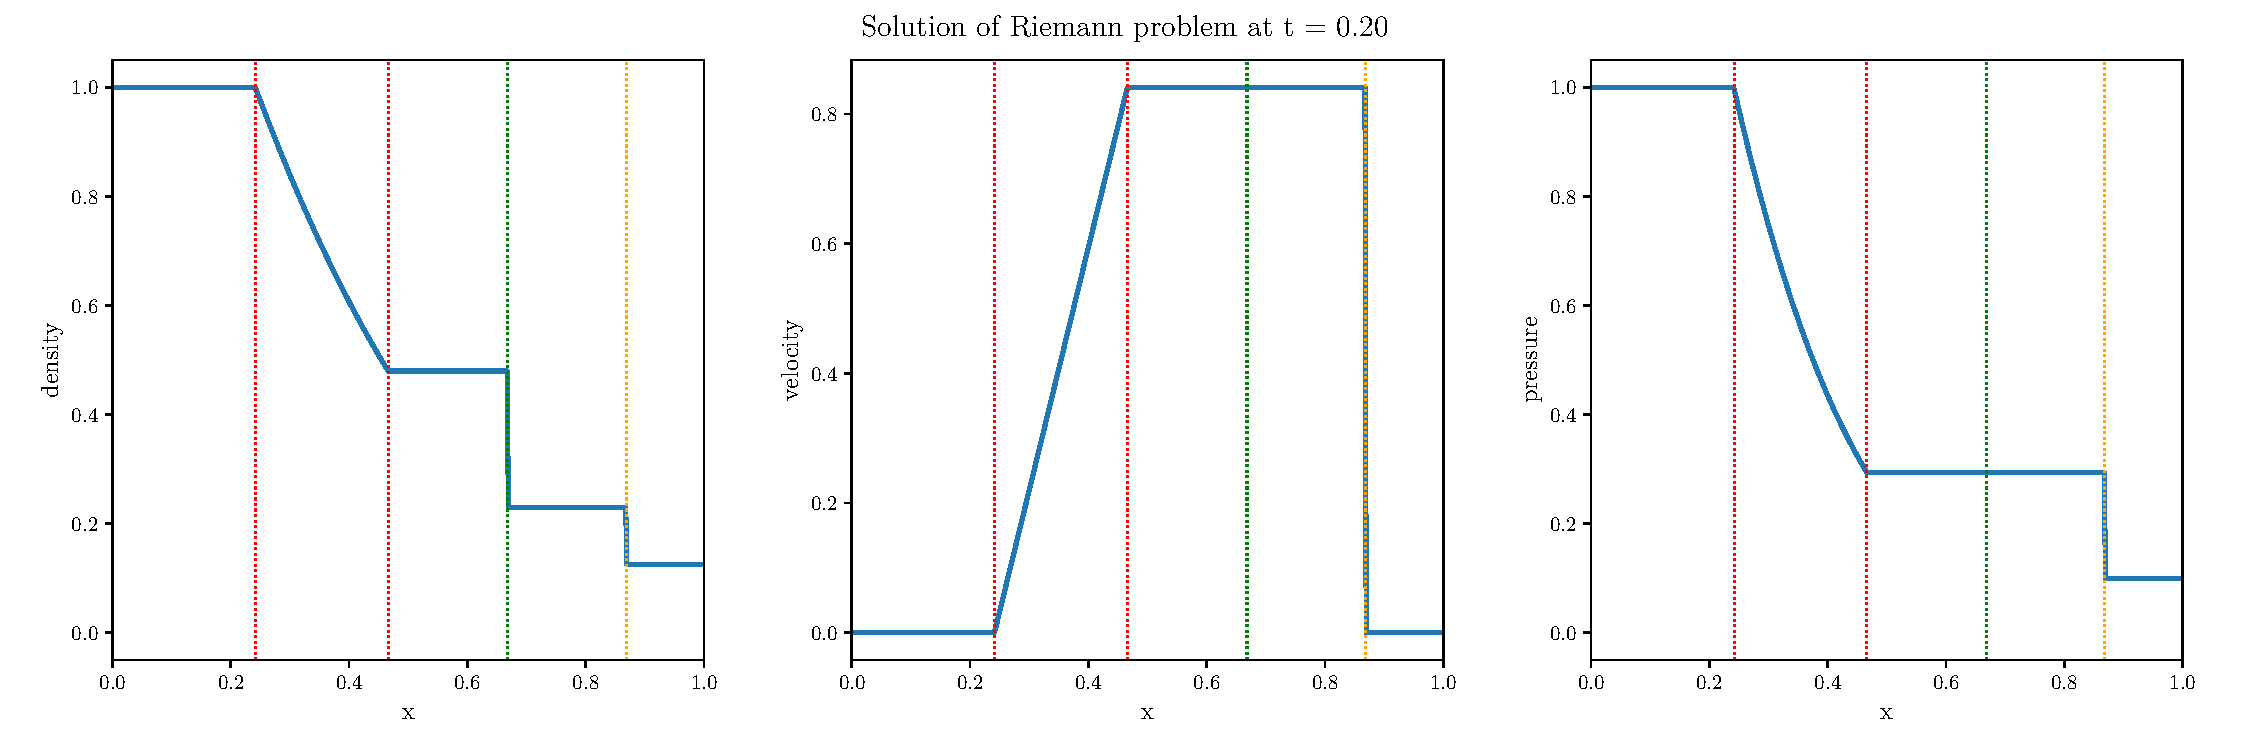
\includegraphics[width=.9\textwidth]{./figures/riemann_exact_solution.pdf}%
	\caption{
		Top row: The initial conditions to a classical Riemann problem, called the Sod shock.\\
%
		Bottom row: The exact solution of the problem at $t = 0.2$.
		The solution consists of a left facing rarefaction wave (between the two red dotted lines), easily recognisable through its non-linear shape.
		To the right (orange dotted line) is a shock wave, across which all three primitive quantities (density, pressure, bulk velocity) change as a jump discontinuity.
		The two waves enclose the third middle wave (green dotted line), which is a contact wave.
		The contact wave is a jump discontinuity just like a shock wave, but only the density changes; Velocity and pressure remain constant.
		\label{fig:riemann-solved}
		}%
\end{figure}















%====================================================================
\subsection{Exact Solver}
%====================================================================


The equation for the pressure in the star region \ref{eq:riemann-pstar} can't be solved analytically, but it can be solved iteratively.

Since we have the analytic function and the first derivative w.r.t. $p$ can be computed, i.e.

\begin{align*}
	\frac{\del f_{L,R}}{\del p} &= 
		\begin{cases}
			\left[ \frac{A_{L,R}}{p + B_{L,R}} \right]^{\frac{1}{2}} \left( 1 - \frac{1}{2} \frac{p - p_{L,R}}{p + B_{L,R}} \right) 
				& ~\text{ if } ~ p > p_{L,R} ~ \quad \text{(shock)} \\
			\frac{a_{L,R}}{\gamma p_{L,R}}  \left( \frac{p}{p_{L,R}} \right)^ \frac{-(\gamma+1)}{2 \gamma}
				& ~\text{ if } ~ p \leq p_{L,R} ~ \quad \text{(rarefaction)} \label{eq:riemann-pstar-dp}\\
		\end{cases} \\
	A_{L,R} &= 
		\frac{2}{(\gamma + 1) \rho_{L,R}}\\
	B_{L,R} &= 
		\frac{\gamma - 1}{\gamma + 1} p_{L,R}
\end{align*}


Then, using the Newton-Raphson iteration, we can find the solution using the prescription

\begin{align}
	p_{n+1} = p_n - \frac{f(p_n)}{\frac{\del f(p_n)}{\del p}}
\end{align}


we re-iterate until it converges, i.e. when the relative pressure change 

\begin{align}
	\frac{|p_k - p_{k+1}|}{\frac{1}{2} | p_k + p_(k+1) | } < \epsilon
\end{align}

where $\epsilon$ is some tolerance. Default value is set in \texttt{defines.h} as \verb|#define EPSILON_ITER 1e-6|.


We need to find a first guess for the pressure. 
An ok way to do it is to take the average:
\begin{align*}
	p_0^* = \frac{1}{2} (p_L + p_R)
\end{align*}

The implemented way is based on a linearised solution based on primitive variables:
\begin{align*}
	p_{PV} &= \frac{1}{2} (p_L + p_R) - \frac{1}{8} (u_R - u_L)(\rho_L + \rho_R)(a_L + a_R)\\
	p_0^* &= \max(\epsilon, p_{PV})
\end{align*}

Note that every step along the iteration, we must make sure that we didn't accidentally get negative pressures, and limit it to zero (or the tolerance $\epsilon$). 
If it drops below zero, it might get stuck there, and then all hell breaks loose.
(Seriously, you will get NANs because you're trying to take fractal powers of negative stuff.)


And that's it for the exact solver.
All that is left to do is sample the solution, which is described in section \ref{chap:sampling-solution}.






%====================================================================
\subsection{Approximate Solvers}
%====================================================================



%====================================================================
\subsubsection{Two-Rarefaction Riemann Solver (TRRS)}
%====================================================================





The big idea is to assume a priori that both the left and right waves are going to be rarefaction waves, and to use that assumption to get an expression for $p^*$ and $u^*$, the pressure and velocity in the star region, respectively.

We get

\begin{align}
	\beta &\equiv 
		\frac{\gamma - 1}{2 \gamma} \\
	u^* &= 
		\frac{
			\frac{2}{\gamma - 1} \left[\left(\frac{p_L}{p_R} \right) ^ \beta - 1\right]+ \frac{u_L}{a_L} \left(\frac{p_L}{p_R} \right) ^ \beta  + \frac{u_R}{a_R}
		}{
			\frac{1}{a_R} + \frac{1}{a_L}\left(\frac{p_L}{p_R} \right) ^ \beta
		} \\
	p^* &=
		\frac{1}{2} \left[
			p_R \left[ \frac{\gamma - 1}{2 a_R} (u^* - u_R) + 1 \right] ^ \frac{1}{\beta} +
			p_L \left[ \frac{\gamma - 1}{2 a_L} (u_L - u^*) + 1 \right] ^ \frac{1}{\beta}
		\right] \label{eq:pstar-trrs}
\end{align}

Note that we may also write $p^*$ independently of $u^*$:

\begin{align}
	p^* = 
		\left[ 
			\frac{ a_L + a_R - \frac{\gamma - 1}{2} (u_R - u_L)}{\frac{a_L}{p_L^\beta} + \frac{a_R}{p_R^\beta}}
		\right] ^ \frac{1}{\beta}
\end{align}

But eq. \ref{eq:pstar-trrs} is computationally more efficient if we compute $u^*$ first. (Way fewer uses of fractional powers.)















%====================================================================
\subsubsection{Two-Shock Riemann Solver (TSRS)}
%====================================================================


The big idea is to assume a priori that both the left and right waves are going to be shock waves, and to use that assumption to get an expression for $p^*$ and $u^*$, the pressure and velocity in the star region, respectively.


The equation for the pressure in the star region (eq. \ref{eq:riemann-pressure-equation}) then is given by

\begin{align}
	f(p) &= (p - p_L) g_L(p) + (p - p_R) g_R(p) + u_R - u_L = 0 \label{eq:riemann-pressure-tsrs} \\
	g_{L,R}(p) &= \left[ \frac{A_{L,R}}{p + B_{L,R}} \right] ^{\half} \\
	A_{L,R} &= 
		\frac{2}{(\gamma + 1) \rho_{L,R}}\\
	B_{L,R} &= 
		\frac{\gamma - 1}{\gamma + 1} p_{L,R}
\end{align}

Unfortunately, this approximation does not lead to a closed form solution.
So we can either use an iterative method again, or use further approximations.
So the idea is to find $p_0$, an estimate for the pressure to use in eq. \ref{eq:riemann-pressure-tsrs}, and to use that to get a better approximation for $p^*$:

\begin{align*}
	p^* = \frac{g_L(p_0) p_L + g_R(p_0)p_R - (u_R - u_L)}{g_L(p_0) + g_R(p_0)}
\end{align*}

and

\begin{align*}
	u^*  = \frac{1}{2} (u_L + u_R) + \frac{1}{2} \left[ (p^* - p_R) g_R(p_0) - (p^* - p_L) g_L(p_0) \right]
\end{align*}


A good choice for $p_0$ is coming from the linearised solution of the primitive variables approach:

\begin{align*}
	p_{PV} &= \frac{1}{2} (p_L + p_R) - \frac{1}{8} (u_R - u_L)(\rho_L + \rho_R)(a_L + a_R)\\
	p_0 &= \max(\epsilon, p_{PV})
\end{align*}










%====================================================================
\subsubsection{HLLC Solver}
%====================================================================


The HLLC solver is based on the approximation that we have 3 waves which are jump discontinuities, travelling with the speeds $S_L$, $S^*$, and $S_R$, respectively.
Using integral relations and Rankine-Hugeniot relations, we directly find an expression for the fluxes $\F$:


\begin{align}
	\F_{i+\half} = \begin{cases}
		\F_L ~~~~ &\text{ if }		~~	\frac{x}{t} \leq S_L \\
		\F^*_L ~~~~ &\text{ if }	~~  S_L \leq \frac{x}{t} \leq S^* \\
		\F^*_R ~~~~ &\text{ if }	~~	S^* \leq \frac{x}{t} \leq S_R \\
		\F_R ~~~~ &\text{ if }		~~	S_R \leq \frac{x}{t} \\
	\end{cases}
\end{align}

where $x/t = 0$ at the boundary of a cell, $i+\half$, and with

\begin{align*}
	S^* &=
		\frac{p_R - p_L  + \rho_L u_L (S_L - u_L) - \rho_R u_R (S_R - u_R)}
			{\rho_L (S_L - u_L) - \rho_R (S_R - u_R) }\\
	\U^*_{L,R} &=
		\rho_{L,R} \frac{ S_{L,R} - u_{L,R}}{S_{L,R} - S^*} 
		\begin{pmatrix}
			1\\
			S^*\\
			v_{L,R}\\
			w_{L,R}\\
			\frac{E_{L,R}}{\rho_{L,R}} + (S^* - u_{L,R}) \left( S^* + \frac{p_{L,R}}{\rho_{L,R}(S_{L,R} - u_{L,R})} \right)
		\end{pmatrix} \\
	\F^*_{L,R} &=
		\F_{L, R} + S_{L,R} ( \U^*_{L,R} - \U_{L,R} )
\end{align*}

for the flux in $x$ - direction;
For $y$ and $z$ direction, you'll need to exchange the velocity components with $S^*$ appropriately.
$\U_{L,R}$ are the given initial states, and $\F_{L,R} = \F(\U_{L,R})$ the corresponding initial states.



What we still lack is estimates for the left and right wave speeds, $S_L$ and $S_R$.
There are multiple ways to get good and robust estimates.
The one I implemented is:

\begin{align}
	S_L  &= u_L - a_L q_L \\
	S_R  &= u_R + a_R q_R \\
	q_{L,R} &= 
		\begin{cases}
			1	~~~~ & \text{ if } p^* \leq p_{L,R} ~~~~ \text{(rarefaction)}\\
			\sqrt{1 + \frac{\gamma + 1}{2 \gamma} \left(\frac{p^*}{p_{L,R}} - 1 \right)}	~~~~ & \text{ if } p^* > p_{L,R} ~~~~ \text{(shock)}\\
		\end{cases} \\
	p^* &= \max(0, p_{PV})\\
	p_{PV} &= \frac{1}{2} (p_L + p_R) - \frac{1}{8} (u_R - u_L)(\rho_L + \rho_R)(a_L + a_R)
\end{align}










%====================================================================
\subsection{Dealing with Vacuum}
%====================================================================


Vacuum is characterized by the condition $\rho = 0$.
With out equation of state, we also have $p = 0$ and $E = 0$ following from $\rho = 0$.
The structure of the solution to the Riemann problem is different, there is no more star region.
It can be shown that a shock wave can't be adjacent to a vacuum.
Instead, we have a rarefaction wave and a contact wave which coalesces with the tail of the rarefaction.
So we have a jump discontinuity next to the vacuum, which makes perfect sense, and this discontinuity will travel with some ``escape velocity'' $u_{vac}$.
Hence it makes sense to characterize the vacuum state as $\mathbf{W}_{vac} = (0, u_0, 0)$.

There are three cases to consider:


\begin{enumerate}

	\item \textbf{The right state is a vacuum:}
	
		The vacuum front travels with the velocity
		\begin{equation}
			S_{vac, L} = u_L + \frac{2 a_L}{\gamma - 1}
		\end{equation}
		and left of it we have a left going rarefaction wave, i.e.
		\begin{align}
			\mathbf{W}_{L, \text{ with vacuum }} = 
				\begin{cases}
					\mathbf{W_L} & \quad \text{ if } \frac{x}{t} \leq u_L - a_L \\
					\mathbf{W_{L, \text{inside fan}}} & \quad \text{ if } u_L - a_L < \frac{x}{t} < S_{vac, L} \\
					\mathbf{W_{vac}} & \quad \text{ if } \frac{x}{t} \geq S_{vac, L}\\
				\end{cases}
		\end{align}
		
	\item \textbf{The left state is a vacuum:}
	
		The vacuum front travels with the velocity
		\begin{equation}
			S_{vac, R} = u_R - \frac{2 a_R}{\gamma - 1}
		\end{equation}
		and right of it we have a right going rarefaction wave, i.e.
		\begin{align}
			\mathbf{W}_{R, \text{ with vacuum }} = 
				\begin{cases}
					\mathbf{W_{vac}} & \quad \text{ if } \frac{x}{t} \leq S_{vac, R}\\
					\mathbf{W_{R, \text{inside fan}}} & \quad \text{ if } S_{vac, R} < \frac{x}{t} <   u_R + a_R\\
					\mathbf{W_R} & \quad \text{ if } \frac{x}{t} \geq u_R + a_R \\
				\end{cases}
		\end{align}
		
	\item \textbf{ Vacuum is being generated }
	
		In certain cases, with both the left and the right state being non-vacuum states, vacuum can be generated in regions of the solution.
		Just think what might happen if the left state has high velocity towards the left, and the right state having a high velocity towards the right, leaving the center region empty.
		The result is that we have a vacuum state emerging around the center, bounded by two vacuum fronts $S_{vac, L}$ on the left side and $S_{vac, R}$ on the right side.
		The full solution is
		\begin{align}
			\mathbf{W} = 
				\begin{cases}
					\mathbf{W}_{L, \text{ with vacuum }} & \quad \text{ if } \frac{x}{t} \leq S_{vac, L}\\
					\mathbf{W}_{vac} & \quad \text{ if } S_{vac, L} < \frac{x}{t} <  S_{vac, R}\\
					\mathbf{W}_{R, \text{ with vacuum }} & \quad \text{ if } \frac{x}{t} \geq S_{vac, R} \\
				\end{cases}
		\end{align}
		
		
		When do we have a vacuum generating condition?
		Well, $S_{vac, L} \leq S_{vac, R}$ must hold, hence
		\begin{align}
			\Delta u_{crit} \equiv \frac{2 a_L}{\gamma - 1 } + \frac{2 a_R}{\gamma - 1 } \leq u_R - u_L
		\end{align}

\end{enumerate}




















%====================================================================
\subsection{Sampling the Solution}\label{chap:sampling-solution}
%====================================================================

With the solvers readily available, the final task is to sample the solution at some given point $(x, t)$.
Assuming we have computed all the star region state variables, what is left to do is to determine in which case the point $(x, t)$ is located.
The flow chart of decision making and finally which relations to use is shown in figure \ref{fig:sampling-solution}.


\begin{sidewaysfigure}
	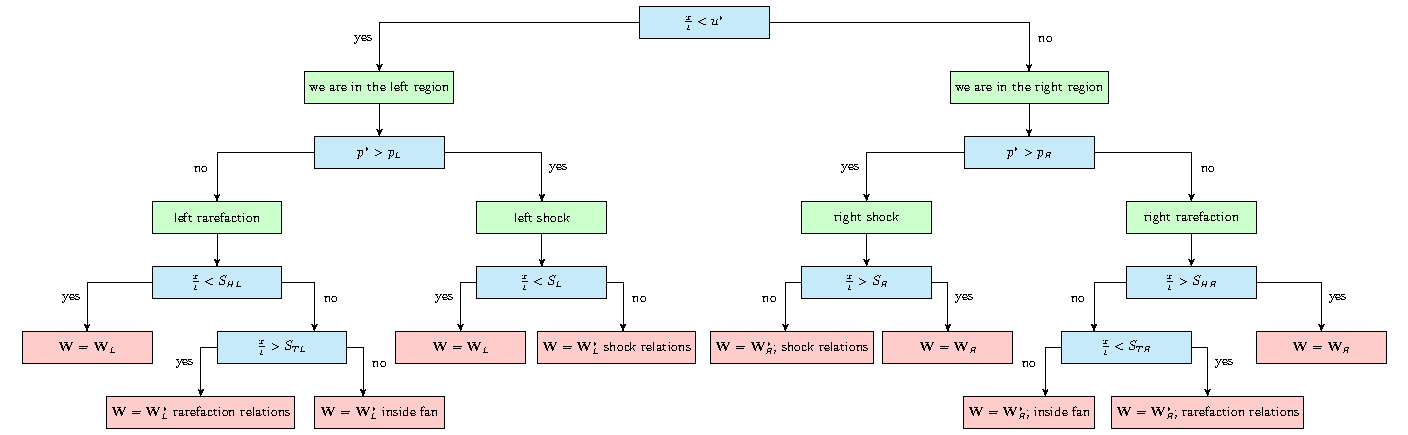
\includegraphics[]{./figures/tikz/sampling_the_solution.pdf}%
	\caption{Flow chart to sample the solution of the Riemann problem for the Euler equations at a given point $(x, t)$.
		\label{fig:sampling-solution}
	}
\end{sidewaysfigure}

Initially all we need to compute is the star states, then we sample the solution at the given point that we're interested in, and the flowchart will tell us which states we need to compute using which relations.










%====================================================================
\subsection{Implementation Details}
%====================================================================


The specific Riemann solvers are \texttt{/program/src/riemann} directory.
If we have a vacuum condition, we always use the vacuum solver, which is given above.
It's not iterative, so no reason to do approximate solutios there.
Note however that for the Godunov method, we may have problems with the vacuum solution.
The vacuum solution of the Riemann problem gives non-zero velocities in regions where $\rho = p = E = 0$.
So if we have for example a left vacuum, until the initial state boundary we will typically have $\U = 0$, while the Riemann problem will give $u \neq 0$ for the flux;
So jump discontinuities will form.

A way to deal with this is to not set the density and pressure to zero, but to a very small number, I employ \texttt{SMALLRHO} and \texttt{SMALLP} in the code, which are defined as macros in \verb|/program/src/defines.h|.
Also, instead of returning a nonzero-velocity in the vacuum, return also something very small, \texttt{SMALLU}.
This makes the code a bit more stable, but it will deviate from the solution of the exact Riemann solver.


However, this exception handling is only used when the code isn't employed as a Riemann solver only.
To differentiate between the cases, the \verb|-DUSE_AS_RIEMANN_SOLVER| flag should be passed to the compiler if you want to run the code as a Riemann solver only.




\newpage

%==============================================
\section{Hydrodynamics Methods}\label{chap:hydro}
%==============================================


%==============================================
\subsection{Godunov's Method}
%==============================================










%============================================
\subsubsection{Method}
%============================================

Godunov's method arises from the integral form of the conservation law so that discontinuous solutions are allowable.

For the one dimensional method, we discretize the spatial domain into $M$ computing cells of regular size, and assume that the initially continuous data is represented by piecewise constant distribution of data, see fig. \ref{fig:piecewise-constant}.



\begin{figure}[H]
	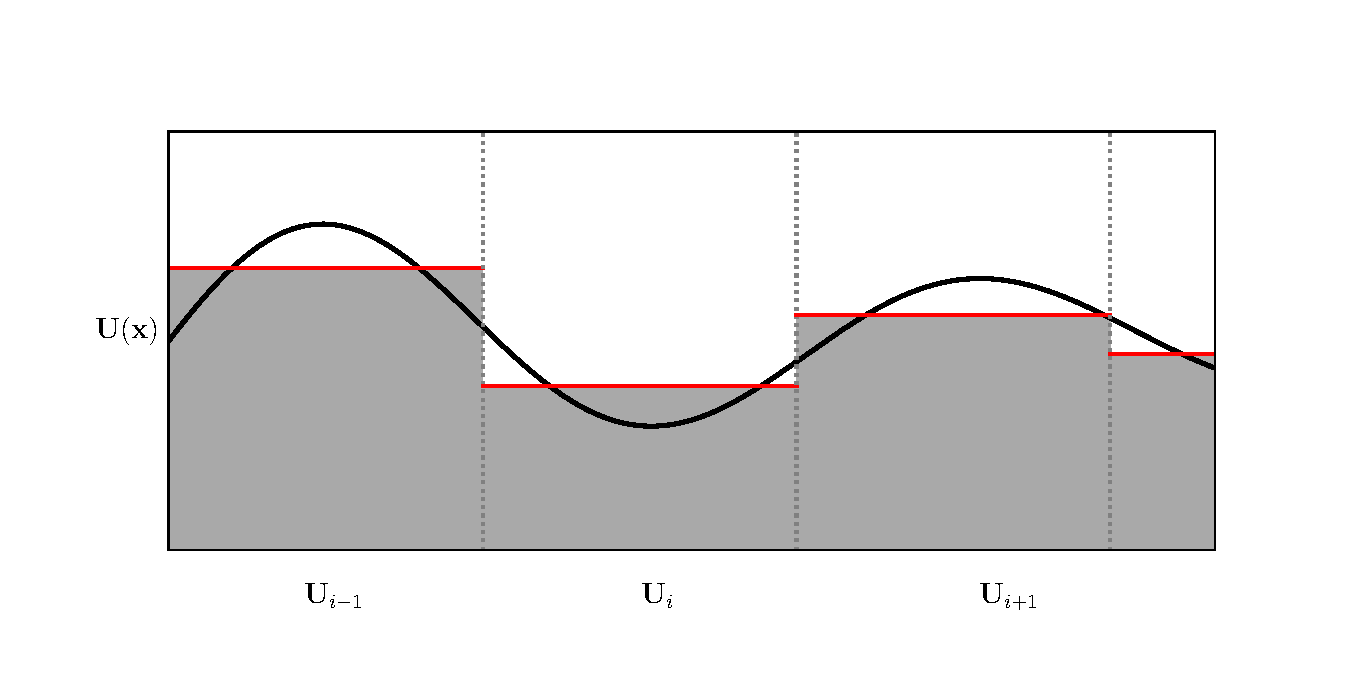
\includegraphics[width=\textwidth]{./figures/piecewise_const.pdf}%
	\caption{	
		A piecewise constant representation of continuous data among cells.
		\label{fig:piecewise-constant}
		}
\end{figure}

Having a collection of piecewise constant states, we effectively have to solve local Riemann problems with data $\U_i$ as $\U_L$ and $\U_{i+1}$ as $\U_R$, centered at the intercell boundary positions $x_{i+\half}$.
The solution of the Riemann problem will depend on $\frac{\bar{x}}{\bar{t}}$, where $\bar{x}$ and $\bar{t}$ are in local coordinates to the specific Riemann problem under consideration. 
$\bar{x}$ is zero at $x_{i+\half}$ and increasingly negative with decreasing $i$.
$\bar{t}$ is zero at the current timestep.


Now suppose that we have solved the Riemann problem at the position $x_{i+\half}$ with left state $\U_L = \U_i$ and right state $\U_R = \U_{i+1}$.
Then, as time evolves, how will the state at $x_{i+\half}$ change?

Recall that the elementary waves travel along characteristics, and that the characteristics are straight lines on the $x-t$ - diagram (see fig. \ref{fig:riemann-solution}.
Then the state at $x_{i+\half}$, which is where the dividing line between the two initial states is, will be given by the solution of the Riemann problem at the position $\bar{x} = 0$, and will remain the same for all $\bar{t} > 0$.
(This is assuming there is nothing else that might disturb the current situation.)


Using that fact, it can be derived that (see \cite{toro}) 

\begin{align}
	\U^{n+1}_i = \U^n_i + \frac{\Delta t}{\Delta x} \left[\F(\U_{i-\half}) - \F(\U_{i+\half}) \right] \label{eq:godunov-discretized}
\end{align}

where $\U_{i-\half}$ and $\U_{i+\half}$ are the solutions to the Riemann problems at $x_{i-\half}$ and $x_{i+\half}$, respectively.


It is noteworthy that this is an exact solution to a piecewise constant initial state.




Lastly, we need to limit the time step size.
We mustn't allow for a wave to be able to travel further than one cell length between two timesteps, otherwise we get bogus results.
Remember that we assumed that the state at $x_{i+\half}$ doesn't change after $\bar{t} > 0$.
This is only satisfied if the wave doesn't reach the boundary of the neighbouring cell.

This time step restriction is imposed by the CFL condition:

\begin{align}
	\Delta t_{max} \leq \frac{C_{cfl} \Delta x}{|S_{max}^n|} \label{eq:godunov-cfl}
\end{align}


where $S_{max}^n$ is the highest wave propagation speed at the current time, and $C_{cfl} \in [0, 1($ is the Courant number.


However, this is not the most practical way of doing things.
In 2D, using dimensional splitting, we'd have to first solve everything in one direction to find the wave speeds, then advance the time step of the sweep, then do the other sweep and hope that the maximal wave velocity won't be greater than the one of the previous sweep.
Or re-do the first sweep iteratively until we get decent time steps.

Instead, we use the estimate

\begin{align}
	S^n_{max} = \max\{ |u_i^n| + a_i^n \}
\end{align}

This is not always accurate, and the wave speed can be underestimated, leading to instabilities.
To combat this, we just need to choose a lower $C_{cfl}$.
Toro recommends to use $C_{cfl} < 0.8 - 0.9$.













%===================================================================
\subsubsection{Implementation Details}\label{chap:godunov-details}
%===================================================================


The cells are stored as an array of \verb|struct cell| that stores both primitive states, \texttt{prim}, as  \texttt{struct pstate}, and conserved states, \texttt{cons}, as \texttt{struct cstate}.
Furthermore they have \texttt{struct pstate pflux} and \texttt{struct cstate cflux} to store fluxes of primitive and conserved variables.


The grid is set up as follows:
In 1D, it is a 1D array of \texttt{struct cell}.
In 2D, it is a 2D array.
Indices (0, 0) represent the lower left corner of the simulation domain.
First index is in x direction, i.e. (nx - 1, 0) is at the coordinates (x = xmax, y = 0).


The flux at $x_{i+\half, j}$ and $y_{i, j+\half}$ are stored in \texttt{cflux} or \texttt{pflux} of cell \verb|grid[i, j]|, depending whether you're storing primitive or conserved variables.
For the Godunov scheme, we need conserved variables.
For advection, we only deal with primitive variables.
Because we're doing dimensional splitting, it suffices to have only one storage place, as they will be used in successive order.
See section \ref{chap:dimensional-splitting} for details.

We can afford to store $x_{i+\half}$ at cell $i$ because we have at least 1 extra virtual boundary cell which is used to apply boundary conditions, so the flux at $x_{-\half}$ will be stored in \verb|grid[BC-1]|, where \texttt{BC} is the number of boundary cells used, defined in \texttt{defines.h}.
 

If the grid is only in 1D, then all the above definitions still apply as if y didn't exist.



The related functions are written in \texttt{/program/src/solver/godunov.c} and \texttt{/program/src/solver/godunov.h}.
The hydro related functions are called in the main loop in \texttt{/program/src/main.c} when \verb|solver_step(...)| is called.

The \verb|solver_step(...)| function does the following for the 1D case:
\begin{itemize}
	\item 	Reset the stored fluxes from the previous timestep to zero
	\item 	Compute the primitive states for all cells from the updated conserved states
	\item 	Impose boundary conditions (section \ref{chap:boundary-conditions})
	\item 	Find the maximal timestep that you can do by applying the CFL condition \ref{eq:godunov-cfl}.
	\item 	Compute fluxes:
	\begin{itemize}
		\item 	For every cell pair $(i, i+1)$, solve the Riemann problem (see section \ref{chap:riemann}) to find the flux $\F_{i+\half}$.
		\item 	Store the flux $\F_{i+\half}$ in the \texttt{struct pstate pflux} struct of the cell $i$.
				\texttt{struct pstate} is a struct that contains the primitive state, i.e. density $\rho$, velocity $u_x$, $u_y$, and pressure $p$.
	\end{itemize}
	\item 	Update the states: Effectively compute $\U^{n+1}$ at this point using $\U_i^n$, the flux $\F_{i+\half}$ stored in every cell $i$, and the flux $\F_{i-\half}$ stored in every cell $i-1$ following eq. \ref{eq:godunov-discretized}.
\end{itemize}

























%==============================================
\subsection{Weighted Average Flux (WAF) Method}
%==============================================







%============================================
\subsubsection{Method}
%============================================


For the WAF method, we again assume piece-wise constant data (see fig. \ref{fig:piecewise-constant}), i.e.

\begin{equation}
	\U_i ^ n = \frac{1}{\Delta \x} \int_{\x_{i-\half}}^{\x_{i+\half}} \U(\x, t^n) \de \x
\end{equation}

The scheme is again based on the explicit conservative formula

\begin{equation}
	\U_{i}^{n+1} = \U_i^n + \frac{\Delta t}{\Delta x} \left[ \F_{i - \half} - \F_{i + \half} \right] \label{eq:hydro_basics_waf}
\end{equation}



The intercell flux $\F_{i + \half}$ is defined as an integral average of the flux function:

\begin{equation}
	\F_{i + \half} = \frac{1}{\Delta x} \int_{-\frac{1}{2} \Delta x} ^{\frac{1}{2} \Delta x} \F (\U_{i+\half} ( x, \frac{1}{2}\Delta t)) \de x \label{eq:hydro-waf-flux}
\end{equation}

The integration range goes from the middle of the cell to the middle of the neighbouring cell.





\begin{figure}[htbp]
	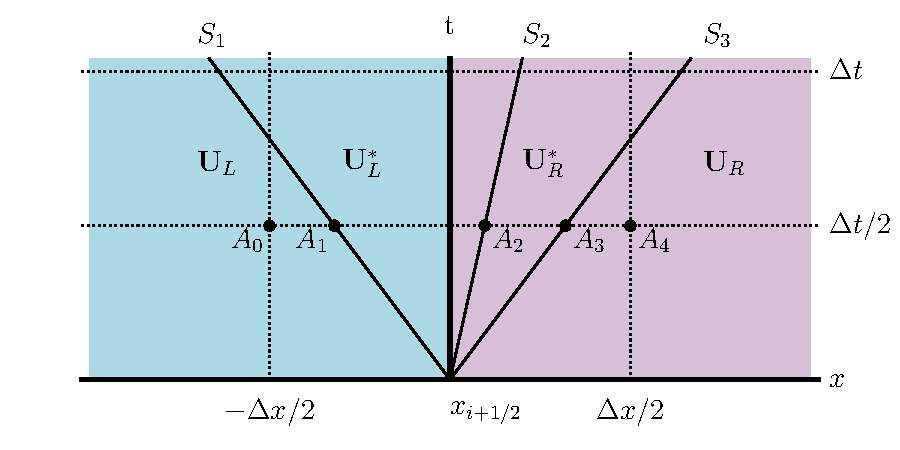
\includegraphics[width=\textwidth]{./figures/WAF-hydro.pdf}%
	\caption{Figure to show the derivation of the WAF intercell flux (eq. \ref{eq:hydro-waf-flux}) for the 1D Euler equations.
		We have initially two piecewise constant states, $\U_i$ and $\U_{i+1}$, separated at the position $x_{i+\half}$.
		As time evolves, three waves will emerge, with respective speeds $S_1$, $S_2$, and $S_3$.
		The states between the points $A_k$, $A_{k+1}$ are assumed constant.
		\label{fig:hydro-waf}
	}
\end{figure}



The solution of the Riemann problem separates the two initial states $\U_L = \U_i$, $U_R = \U_{i+1}$ into four states

\begin{align*}
	\U^{(1)} = \U_L, \quad	\U^{(2)} = \U_L^*, \quad	\U^{(3)} = \U_R^*, \quad	\U^{(4)} = \U_R
\end{align*}

that are separated by three waves with the speeds $S_1$, $S_2$, and $S_3$.
At $t = \frac{1}{2} \Delta t$, we can separate the interval $[-\Delta x /2, \Delta x /2]$ by introducing 5 points along the $x$ axis:

\begin{align*}
	A_0 &= - \Delta x / 2\\
	A_1 &= S_1 \Delta t / 2\\
	A_2 &= S_2 \Delta t / 2\\
	A_3 &= S_3 \Delta t / 2\\
	A_4 &= \Delta x / 2
\end{align*}

and separate the integral \ref{eq:hydro-waf-flux} into the sum
\begin{align}
\F_{i + \half} = \frac{1}{\Delta x} \sum\limits_{k = 1}^{N+1} \int\limits_{A_{k-1}}^{A_k} \F (\U(x, \Delta t / 2)) \de x
\end{align}

where $N$ is the number of occuring waves in the solution.





Note that with $|C_{cfl}| \leq 1$ we should always have all the waves within $[-\Delta x /2, \Delta x / 2]$ at $t = \Delta t / 2$ if the $C_{cfl}$ is chosen properly using actual wave speeds.
However, we use approximate wave speed estimates, so we need to check whether the actual waves are still inside $[-\Delta x /2, \Delta x / 2]$ at $t = \Delta t / 2$.



Since we assume constant states between these points (which they will be unless we have a rarefaction present), the fluxes $\F$ between the points $A_k$ will be constant too, and the integral is trivial.
We only need expressions for the distances $\overline{A_{k}A_{k+1}}$.
It's easy to show that regardless of the sign of the wave speeds $S_k$, we obtain

\begin{align*}
	\overline{A_0 A_1} &= 
		\frac{\Delta x}{2} ( 1 + c_1 ) \\
	\overline{A_1 A_2} &= 
		\frac{\Delta x}{2} ( c_2 - c_1 ) \\
	\overline{A_2 A_3} &= 
		\frac{\Delta x}{2} ( c_3 - c_2 ) \\
	\overline{A_3 A_4} &= 
		\frac{\Delta x}{2} ( 1 - c_3 ) \\ 
	\text{ with } c_k &= \frac{S_k \Delta t}{\Delta x}
\end{align*}



If we define

\begin{align*}
	\beta_k &= \frac{\overline{A_{k-1} A_k}}{\Delta x}\\
	c_0 &= -1, \quad c_5 = c_{N+1} = 1
\end{align*}

we obtain

\begin{align*}
	\beta_k &= \frac{1}{2} (c_k - c_{k-1})
\end{align*}

and we can write the WAF flux as

\begin{align}
	\F_{i + \half} 
		&= \sum\limits_{k = 1}^{N+1} \beta_k \F^{(k)} \\
		&= \frac{1}{2} (\F_i + \F_{i+1}) - \frac{1}{2} \sum\limits_{k = 1}^{N} c_k \left (\F^{(k+1)} - \F^{(k)} \right) 
\end{align}




The TVD modification of the WAF flux is


\begin{align}
	\F_{i + \half} 
		&= \frac{1}{2} (\F_i + \F_{i+1}) - \frac{1}{2} \sum\limits_{k = 1}^{N} sign(c_k) \psi_{i+\half}^{(k)} \left (\F^{(k+1)} - \F^{(k)} \right) \\
	\psi_{i+\half}^{(k)}
		&= \psi_{i+\half}(r^{(k)}) \\
	r^{(k)} &=
		\begin{cases}
			\frac{\Delta q_{i-\half}^{(k)}}{\Delta q_{i+\half}^{(k)}}	& \text{ if } c_k > 0 \\[2em]
			\frac{\Delta q_{i+3/2}^{(k)}}{\Delta q_{i+\half}^{(k)}}	& \text{ if } c_k < 0 \\		
		\end{cases}
\end{align}

Where $q$ is one single quantity which is known to change across every wave.
Options are density $\rho$ and internal energy $\epsilon$.
I implemented the choice $\rho$.

The notation here is a bit tricky: $k$ signifies which wave in the solution of Riemann problems (not only one Riemann problem!!) we look at:

\begin{itemize}
	\item $\Delta q_{i+\half}^{(k)}$ is the jump in e.g. density between wave $k$ and $k + 1$ of the solution of the Riemann problem with initial conditions $\U_L = \U_i$, $\U_R = \U_{i+1}$
	\item $\Delta q_{i-\half}^{(k)}$ is the jump between wave $k$ and $k+1$ of the solution of the Riemann problem with initial conditions $\U_L = \U_{i-1}$, $\U_R = \U_{i}$
	\item $\Delta q_{i+3/2}^{(k)}$ is the jump between wave $k$ and $k+1$ of the solution of the Riemann problem with initial conditions $\U_L = \U_{i+1}$, $\U_R = \U_{i+2}$
\end{itemize}

See figure \ref{fig:WAF-delta-q} for visual clarification.



\begin{figure}[htpb]
	\centering
	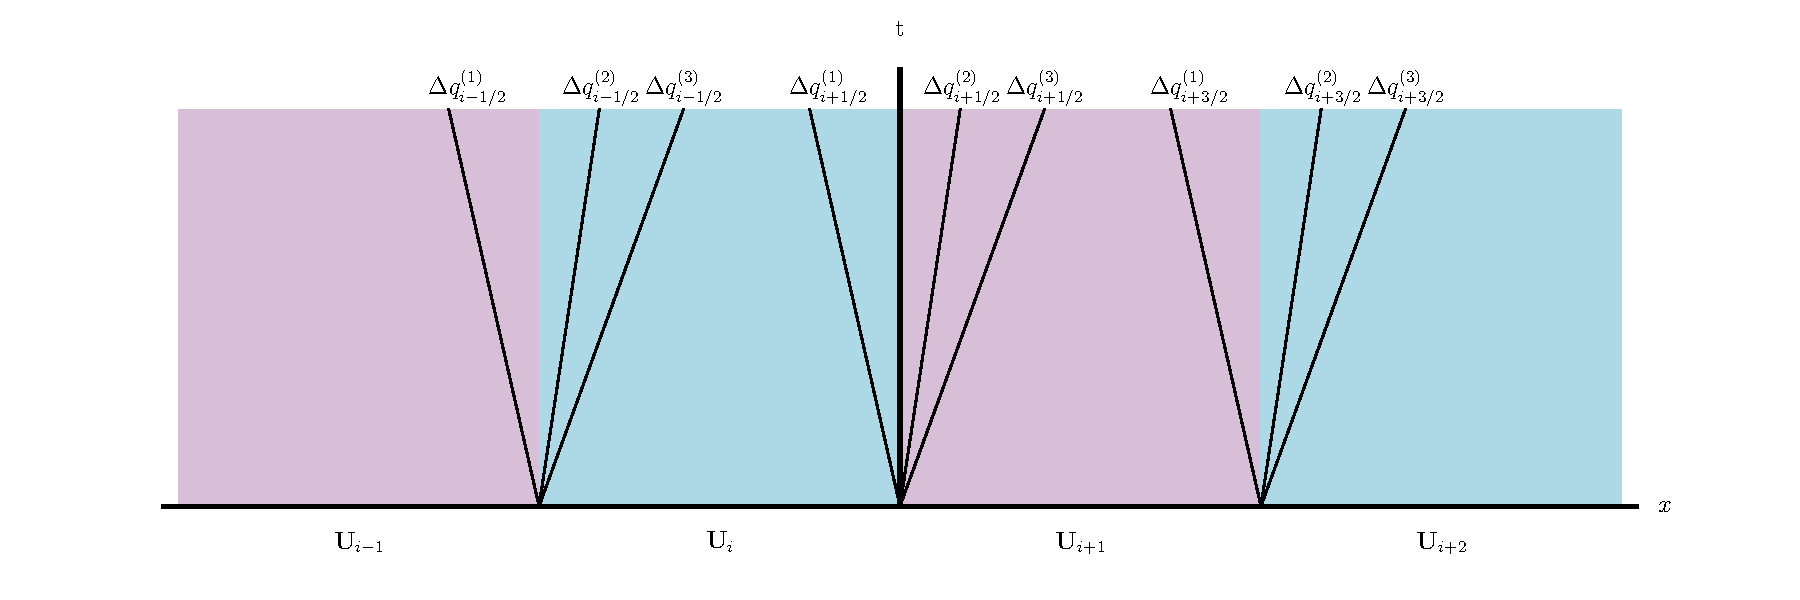
\includegraphics[width=\textwidth]{figures/WAF-hydro-delta-q.pdf}%
	\caption{
		Clarification of the value differences $\Delta q _{i}^{(k)}$ needed to compute the flow parameter $r$ for the WAF method.
		\label{fig:WAF-delta-q}
	}
\end{figure}



The limiters $\psi$ are related to conventional flux limiters $\phi$ via

\begin{equation}
	\psi_{i+\half} = 1 - ( 1 - |c|) \phi_{i+\half}(r)
\end{equation}

Some implemented options are given in section \ref{chap:implemented_limiters}.












%===================================================================
\subsubsection{Dealing with Vacuum}\label{chap:hydro-WAF-vacuum}
%===================================================================


Vacuum needs some special attention because it doesn't follow the solution structure of a typical Riemann problem.
It can easily crash your program:
Consider for example the computation of the local sound speed $a = \sqrt{\gamma p/\rho}$ for $\rho = 0$.
There is no more star region present, instead next to the vacuum ($\rho = 0$) we have a contact wave coinciding with the tail of a rarefaction wave - a wave that we also handle only approximately.

I wasn't able to find literature of how to best deal with this, but I was able to find an approximate solution on my own following the idea of how the WAF scheme works.

In the end, what we want is a solution that we can use to get WAF fluxes, namely we need

\begin{itemize}
	\item 4 fluxes $\F_{i}^{(k)}$ corresponding to the four states $\U_{i}^{(k)}$: $U_L$, $U_L^*$, $U_R^*$, $U_R$
	\item 3 wave speeds $S_L$, $S^*$, $S_R$
	\item 3 differences/jumps in density $q^{(k)}$: $\rho_L^* - \rho_L$, $\rho_R^* - \rho_L^*$, $\rho_R - \rho_R^*$
\end{itemize}

For vacuum, we have three cases to consider, where $\U_{vac}$ describes the vacuum state:


\begin{enumerate}

	\item 	\textbf{The right state is a vacuum}:
	
			Choose 
			\begin{align*}
				\F^{(1)} &= \F(\U_L)\\
				\F^{(2)} &= \begin{cases}
								&\F(\U(t = \Delta t/2, \ x = 0) \quad \text{ for a sonic rarefaction } \\
								&\F(\U_L) \quad \text{ for a non-sonic rarefaction } \\
							\end{cases}\\
				\F^{(3)} &= \F(\U_{vac})\\
				\F^{(4)} &= \F(\U_R)\\[.5em]
				S^{(1)} &= 0\\
				S^{(2)} &= \text{ rarefaction tail speed}\\
				S^{(3)} &= \text{ rarefaction head speed}\\[.5em]
				q^{(1)} &= \rho^*_L - \rho_L\\
				q^{(2)} &= 0\\
				q^{(3)} &= 0\\							
			\end{align*}
			
			Where $\rho^*_L$ is either the density of $\U_L$ or of $\U(x = 0, t = \Delta t/2)$, depending on whether we have a sonic or non-sonic rarefaction.

	
	\item 	\textbf{The left state is a vacuum}:
			
			Choose 
			\begin{align*}
				\F^{(1)} &= \F(\U_L)\\
				\F^{(2)} &= \F(\U_{vac})\\
				\F^{(3)} &= \begin{cases}
								&\F(\U(t = \Delta t/2, \ x = 0) \quad \text{ for a sonic rarefaction } \\
								&\F(\U_R) \quad \text{ for a non-sonic rarefaction } \\
							\end{cases}\\
				\F^{(4)} &= \F(\U_R)\\[.5em]
				S^{(1)} &= 0\\
				S^{(2)} &= \text{ rarefaction tail speed}\\
				S^{(3)} &= \text{ rarefaction head speed}\\[.5em]
				q^{(1)} &= 0\\
				q^{(2)} &= 0\\
				q^{(3)} &= \rho_R - \rho_R^*\\							
			\end{align*}
			
			Where $\rho^*_R$ is either the density of $\U_R$ or of $\U(x = 0, t = \Delta t/2)$, depending on whether we have a sonic or non-sonic rarefaction.
			
	
	\item 	\textbf{A vacuum is being generated}:
	
			This may occur when condition \ref{eq:vacuum-generating-condition} is satisfied.
			The solution structure contains two rarefaction fans, to the left and to the right, enclosed by the initial states $U_L$ and $U_R$, and separated by a vacuum state $U_{vac}$.
			
			My solution strategy is as follows:
			Compute an approximate solution to describe the average state inside each rarefaction fan, and then ``stretch'' the states out such that we pretend that there is no vacuum state in between.
			
			For example, for the left star state, we can compute the rarefaction head speed $S_{L,H}$ and tail speed $S_{L,T}$ and define the average speed $\overline{S}_L = \frac{S_{H,L} + S_{T,L}}{2}$.
			
			Now we approximate the entire star state as the solution inside a rarefaction fan, eqns. \ref{eq:rho-rarefaction-fan-left}-\ref{eq:pressure-rarefaction-fan-left} and \ref{eq:rho-rarefaction-fan-right}-\ref{eq:pressure-rarefaction-fan-right}, at $x/t = \overline{S}_L$.
			The same computation can be done for the right rarefaction.
			
			Then we say that we have no vacuum state in between, but instead ``stretch out'' the star states to meet at a contact wave with speed $S^* = \frac{S_{T,L} + S_{T,R}}{2}$.
			However, we want the total mass, momentum, and energy to be conserved.
			Hence we need to reduce the density, momentum, and energy by a factor
			\begin{align*}
				f_{L,R} = \frac{S_{HL,R} - S_{L,R}}{S_{HL,R} - \frac{S_L + S_R}{2}}
			\end{align*}
			which is simply the ``stretch factor'' based on the distances the utilized waves would travel at any given time $t > 0 $.
			
			In terms of primitive variables, it suffices to apply this factor to density and pressure such that energy, momentum, and mass conservation are satisfied.
			With this, we have expressions for the two star states and a contact speed $S^*$, and can now easily compute the four necessary fluxes.
			
			This solution is not very good, because even when applying flux limiters, it will introduce new peaks at the position of the vacuum.
			However, due to the lack of a better idea, this is what we have.
			At least it provides a somewhat usable solution, such that the WAF method can be used in actual hydrodynamics applications without worrying of code crashes should such a condition occur even for very small time steps.
			

\end{enumerate}
























%===================================================================
\subsubsection{Implementation Details}\label{chap:hydro-WAF-details}
%===================================================================



%===========================================
\section{Slope and Flux Limiters}
%===========================================







%===================================================
\subsubsection{Effects on linear advection}
%===================================================


\quickfigcap
	{./figures/limiters/limiter_comparison.png}
	{fig:limiters-advection}
	{The effect of different slope limiters on linear advection, applied to piecewise linear advection (eqns \ref{eq:advection}, \ref{eq:advection-slope})}




\begin{itemize}

	\item All limiters except superbee still contain diffusion. You can't get rid of it entirely, but we got rid of the oscillations.
	
	\item The minmod resembles the solution of the piecewise constant advection, but pay attention that this is at much later times!
	
	\item Some limiters flatten continuous maxima. Van leer, then MC, then superbee in order of ascending ``flattening''
	
	\item It's as if superbee tries to produce jump discontinuities
	
	\item For order of convergence study, see figs. \ref{fig:advection-convergence-dx-gaussian} - \ref{fig:advection-convergence-CFL-step}, and discussion in section \ref{chap:advection-conclusions}.

\end{itemize}







\newpage
\section{Boundary Conditions}



\begin{figure}[htbp]
	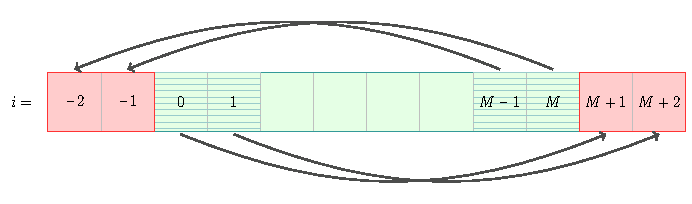
\includegraphics[width=\textwidth]{./images/tikz/boundary_periodic.pdf}%
	\caption{\label{fig:boundary_periodic}
		Method to obtain periodic boundary conditions.
		The ghost cells are red, the arrows show what will be copied where.
	}
\end{figure}



\begin{figure}[htbp]
	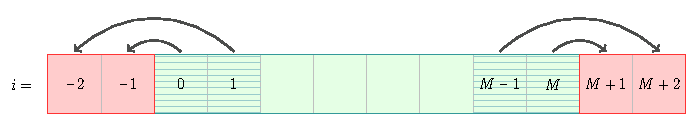
\includegraphics[width=\textwidth]{./images/tikz/boundary_wall.pdf}%
	\caption{\label{fig:boundary_wall}
		Method to obtain wall boundary conditions.
		The ghost cells are red, the arrows show what will be copied where.
	}
\end{figure}



\begin{figure}[htbp]
	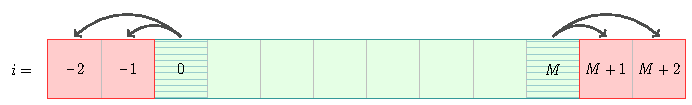
\includegraphics[width=\textwidth]{./images/tikz/boundary_transmissive.pdf}%
	\caption{\label{fig:boundary_transmissive}
		Method to obtain transmissive boundary conditions.
		The ghost cells are red, the arrows show what will be copied where.
	}
\end{figure}



There are tricks how to obtain different kinds of boundary conditions.
In every case, we add additional cells (``\emph{ghost cells}'') in every dimension so we can simulate the desired behaviour.
How many cells you need to add depends on the methods (and mostly stencils) you use.
If you only take into account one neighbouring cell, then one ghost cell on every boundary suffices.
In figures \ref{fig:boundary_periodic}, \ref{fig:boundary_wall}, and \ref{fig:boundary_transmissive}, two ghost cells for a 1D grid are drawn.


Suppose we have 1D grid with $M$ cells and require 2 ghost cells each, which will have indices $-2$, $-1$, $M+1$, and $M+2$.
Then we can get:

\begin{itemize}
	\item \textbf{periodic boundary conditions:}
	
		what goes over the right edge, comes back in over the left edge, and vice versa.
		We achieve this behaviour by enforcing (fig. \ref{fig:boundary_periodic})
		\begin{align*}
			\U_{-2} &= \U_{M-1} \\
			\U_{-1} &= \U_{M}	\\
			\U_{M+1} &= \U_0 	\\
			\U_{M+2} &= \U_1 	\\
		\end{align*}
		
		
		
	\item \textbf{reflective boundary conditions:}
	
		pretend there is a wall at the boundary. 
		We achieve that by ``mirroring'' the cells next to the boundary (fig \ref{fig:boundary_wall}):

		\begin{align*}
			\U_{-2} &= \U_1		\\
			\U_{-1} &= \U_0		\\
			\U_{M+1} &= \U_{M}	\\
			\U_{M+2} &= \U_{M-1}\\
		\end{align*}
		
		However, every directional component (i.e. velocities/momentum) needs to have the negative value in the ghost cell compared to the real cell.
	
	
	\item \textbf{transmissive boundary conditions}:
	
		Just let things flow out however they want. 
		We achieve this by copying the last boundary cell over and over again, such that it looks that the fluid appears to have that state infinitely, and there are no net fluxes to interfere with the hydrodynamics inside the actual grid (fig. \ref{fig:boundary_transmissive})
		
		
		\begin{align*}
			\U_{-2} &= \U_0		\\
			\U_{-1} &= \U_0		\\
			\U_{M+1} &= \U_{M}	\\
			\U_{M+2} &= \U_{M}	\\
		\end{align*}	
	
\end{itemize}




\newpage
\section{Dimensional Splitting}


To go from one to multiple dimensions, it is tempting to just extend the one dimensional discretisation.
For example, starting with the conservation law

\begin{equation}
	\deldt{\U} + \deldx{\F(\U)} + \frac{\del}{\del y} \mathbf{G}(\U) = 0
\end{equation}


and just apply Godunov's finite volume method:

\begin{equation}
	\U_{i,j}^{n+1} = 
					\U_{i,j}^n 
					+ \frac{\Delta t}{\Delta x} \left( \F_{i - \half, j} - \F_{i + \half, j}\right) 
					+ \frac{\Delta t}{\Delta x} \left( \mathbf{G}_{i ,j - \half} - \mathbf{G}_{i, j + \half}\right) 
\end{equation}


However, this is a bit of a problem.
The upwinding here is not complete.
Consider the 2D advection equation

\begin{equation}
	\deldt{q} + u\deldx{q} + v \frac{\del}{\del y} q = 0
\end{equation}

Now suppose we have advecting velocities $u = v = 1$, i.e. the advection velocity is along the diagonal.
Then our method reads 

\begin{equation}
	q_{i,j}^{n+1} = 
					q_{i,j}^n 
					+ u \frac{\Delta t}{\Delta x} \left( q_{i - \half, j} - q_{i + \half, j}\right) 
					+ v \frac{\Delta t}{\Delta x} \left( q_{i ,j - \half} - q_{i, j + \half}\right) 
\end{equation}

This expression doesn't involve $q_{i-1, j-1}$ at all, but that's actually the value that should be advected to $q_{i, j}$ in the next timestep!


One way of doing things is to actually formulate more sophisticated unsplit methods that involve the appropriate stencils.
We shan't do that here though.
We make use of dimensional splitting. 
Instead of solving

\begin{equation}
	\begin{cases}
		\text{PDE: } & \deldt{\U} + \deldx{\F(\U)} + \frac{\del}{\del y} \mathbf{G}(\U) = 0\\
		\text{IC: } & \U(x, y, t^n) = \U^n
	\end{cases}
\end{equation}

we do it in 2 (3 for 3D) steps:

Step 1: We obtain a intermediate result $\U^{n+\half}$ by solving the ``x - sweep'' over the full time interval $\Delta t$ :
\begin{equation}
	\begin{cases}
		\text{PDE: } & \deldt{\U} + \deldx{\F(\U)} = 0\\
		\text{IC: } &  \U^n
	\end{cases}
\end{equation}

and then we evolve the solution to the final $\U^{n+1}$ by solving the ``y - sweep'' over the full time interval $\Delta t$ :

\begin{equation}
	\begin{cases}
		\text{PDE: } & \deldt{\U} + \frac{\del}{\del y} \mathbf{G}(\U) = 0\\
		\text{IC: } & \U^{n+\half} \\
	\end{cases}
\end{equation}

using the 1D methods that are described.

What's even better is that it can be shown (see \cite{leveque_2002}) that by switching the order of the sweeps every timestep (and keeping the time step interval $\Delta t$ constant) leads to a second order accurate method in time.
This is called ``Strang splitting''.

















\newpage
\section{Advection}

\subsection{Analytical Equation}

Advection is a bit of an exception as a hydrodynamics method because we're not actually solving the (ideal) gas equations, but these instead:

\begin{equation}
	\DELDT{ \U } + v \cdot \DELDX{\U} = 0
\end{equation}


Which is still a conservation law of the form

\begin{equation}
	\DELDT{ \U } + \DELDX{\F} = 0
\end{equation}

with the flux tensor 

\begin{equation}
	\F = v \cdot \U
\end{equation}

We assume the advection velocity $v = $ const.

Note that in the formalism used, we only solve the 1D advection, but for every component of the state vector $\U$ and flux tensor $\F$

The analytical solution is given by any function $q(x)$ with $\U(x,t) = q(x - v t)$, which is just $q(x)$ translated by $v t$.




\subsection{Piecewise Constant Method}

\begin{figure}[htbp]
	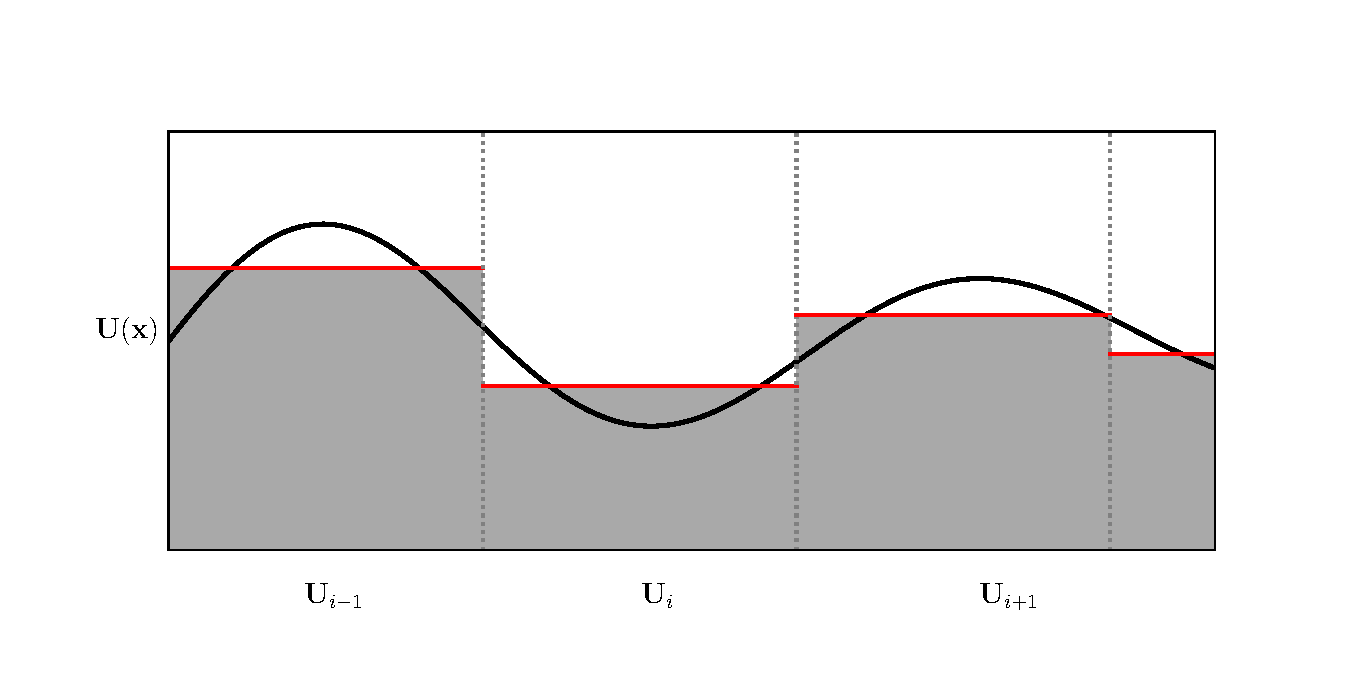
\includegraphics[width=\textwidth]{./figures/piecewise_const.pdf}%
	\caption{Piecewise constant reconstruction of the field
		\label{fig:pwconst}
	}
\end{figure}


We assume that the cell state within a cell is constant (fig. \ref{fig:pwconst}).
Furthermore, we also assume that the velocity $v$ is constant and positive.


\begin{align}
	\U_i ^{n+1} &= 
		\U_i^{n} +  \frac{\Delta t}{\Delta x} \left( \F_{i-\half}^{n+\half} - \F_{i+\half}^{n+\half} \right) \label{eq:advection_basic}\\ 
	\F_{i\pm\half}^{n+\half} &= v_{i\pm\half}\cdot \U_{i - \half \pm \half} \label{eq:advection_flux}
\end{align}

The method is first order accurate in time and space.





We assumed that the velocity is positive and constant.
What if it's negative?

The important point is that we always do \textbf{downwind differencing}.
To obtain a finite difference, as we do here, you must never use the value that is downstream, i.e. that is in the direction of the flux.
Doing this means taking a value for your computation that won't be valid as soon as an infinitesimal time interval passes, because the ingoing flux will change the downwind state.
This is unphysical and leads to violent instabilites.

So if we have negative velocity, all we need to do is change the expression \ref{eq:advection_flux} to

\begin{equation}
	\F_{i\pm\half}^{n+\half} = v_{i\pm\half}\cdot \U_{i + \half \pm \half}
\end{equation}









\subsection{Piecewise Linear Method}

\begin{figure}[htbp]
	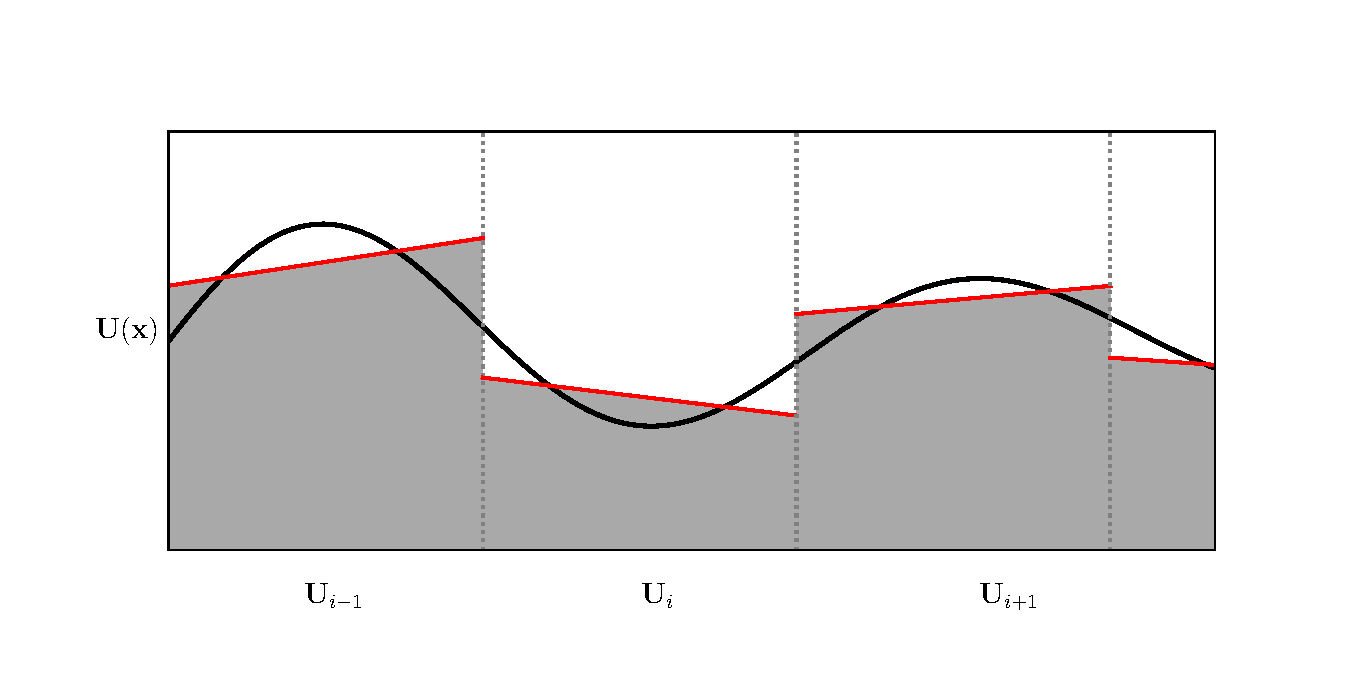
\includegraphics[width=\textwidth]{./figures/piecewise_linear.pdf}%
	\caption{Piecewise linear reconstruction of the field
		\label{fig:pwlin}
	}
\end{figure}



This time, we assume that the state is not constant within a cell, but follows a piecewise linear profile with some slope $\mathbf{s}$ (fig. \ref{fig:pwlin}):

\begin{align*}
	\text{For } x_{i-\half} < x_i < x_{i+\half}: &&
	\quad \U(x, t=t_n) &= \U_i^n + \mathbf{s}_i^n(x - x_i) \\
	\text{Centered method:} && \mathbf{s_i}^n &= \frac{\U_{i+1}^n - \U_{i-1}^n}{ 2 \Delta x}
\end{align*}

Other choices for the slope are possible and stable.




Assuming a positive constant velocity $v$, we derive the flux $\F$ at the time $t^n < t < t^{n+1}$ at the interface position $i-\half$.
At time $t$, the cell will have been advected by a distance $v (t - t^n)$, and the the current state at the interface will be

\begin{align*}
	\U(x=x_{i-\half}, t) 
		&= \U_{i-1}^n + \mathbf{s}_{i-1} (x_{i-\half} - v (t - t^n) - x_{i-1}) \\
		&= \U_{i-1}^n + \mathbf{s}_{i-1} (\frac{1}{2} \Delta x - v (t - t^n))
\end{align*}

To understand how the $x_{i-\half} - v (t - t^n)$ comes into play, imagine the state doesn't change (i.e. isn't advected), but you move the boundaries to the left instead over a distance $v(t - t^n)$.

So if we have a \textbf{negative} constant velocity, the term changes to 

\begin{align*}
	\U(x=x_{i-\half}, t) 
		&= \U_{i}^n + \mathbf{s}_{i} (x_{i-\half} - v (t - t^n) - x_{i}) \\
		&= \U_{i}^n + \mathbf{s}_{i} (-v (t - t^n) - \Delta x)
\end{align*}



Note that the minus sign remains, and that the indices changed by one because we need to always make sure to do upwind differencing, i.e. take only values where the flow comes from, not from the direction where it's going.

Finally, we can compute the average flux over the time step $\Delta t = t^{n+1} - t^{n}$:
\begin{align}
	\F_{i-\half}^{n+\half} 
	&= \langle \F_{i+\half}(t)\rangle _{t^n} ^ {t^{n+1}} 
	= \frac{1}{\Delta t} \int_{t^n}^{t^{n+1}} v \U(x 
	= x_{i-\half}, t) \\
	&= \frac{1}{\Delta t} \int_{t^n}^{t^{n+1}} v \left( \U_{i-1}^n + \mathbf{s}_{i-1} (\frac{1}{2} \Delta x - v (t - t^n)) \right) \\
	&= v \left( \U_{i-1}^n  + \mathbf{s}_{i-1} \left( \frac{1}{2} \Delta x - v \left( \left[ \frac{1}{2 \Delta t} t^2 \right]_{t^n}^{t^{n+1}} - t^n \right)  \right) \right) \\
	&= v \left( \U_{i-1}^n  + \mathbf{s}_{i-1} \left( \frac{1}{2} \Delta x - v \left[ \frac{1}{2} (t^{n+1} + t^n) - t^n \right] \right) \right) \\
	&= v \left( \U_{i-1}^n  + \frac{1}{2} \mathbf{s}_{i-1} \left(\Delta x - v \Delta t \right) \right)
\end{align}



Finally averaging the fluxes over a time step gives:
\begin{equation}
	\U_i^{n+1} = \U_i^n - v \cdot \frac{\Delta t}{\Delta x} ( \U_i ^n - \U_{i-1}^n) - v \cdot \frac{\Delta t}{\Delta x} \frac{1}{2} (\mathbf{s}_i^n - \mathbf{s}_{i-1}^n)(\Delta x - v \Delta t)
\end{equation}

This is the same as eq. \ref{eq:advection_basic} where we used
\begin{align*}
	\F_{i + \half}^{n+\half} 
		& = v_{i+\half} \cdot  \U_{i+\half} ^{n + \half} \\
		& = v \cdot \U(x_{i+\half} - \frac{1}{2} v \Delta t) \\
		& = v \cdot \left( \U_i^n + \mathbf{s}_i^n [(x_{i+\half} - \frac{1}{2} v \Delta t) - x_i ]  \right)\\
		& = v \cdot \left( \U_i^n + \frac{1}{2} \mathbf{s}_i^n (\Delta x -  v \Delta t)  \right)\\
\end{align*}

and analoguely
\begin{align*}
	\F_{i - \half}^{n+\half} 
		& = v \cdot \left( \U_{i-1}^n + \frac{1}{2} \mathbf{s}_{i-1}^n (\Delta x -  v \Delta t)  \right)\\
\end{align*}








To summarize the formulae:

\begin{align*}
	\U_i ^{n+1} &= 
		\U_i^{n} +  \frac{\Delta t}{\Delta x} \left( \F_{i-\half}^{n+\half} - \F_{i+\half}^{n+\half} \right) & \\
	\F_{i-\half}^{n+\half} &= 
		\begin{cases}
			v_{i-\half} \cdot \U_{i-1}^n +  \frac{1}{2} v_{i-\half} \cdot\mathbf{s}_{i-1}^n (\Delta x -  v_{i-\half} \Delta t)
			 	& \quad \text{for } v \geq 0 \\
			v_{i-\half} \cdot \U_{i}^n -\frac{1}{2} v_{i-\half} \cdot \mathbf{s}_{i}^n (\Delta x + v_{i-\half} \Delta t)
				& \quad \text{for } v \leq 0 \\
		\end{cases} \\
	\F_{i+\half}^{n+\half} &= 
		\begin{cases}
			v_{i+\half} \cdot \U_{i}^n +  \frac{1}{2} v_{i+\half} \cdot\mathbf{s}_{i}^n (\Delta x -  v_{i+\half} \Delta t)
			 	& \quad \text{for } v \geq 0 \\
			v_{i+\half} \cdot \U_{i+1}^n -\frac{1}{2} v_{i+\half} \cdot \mathbf{s}_{i+1}^n (\Delta x + v_{i+\half} \Delta t)
				& \quad \text{for } v \leq 0 \\
		\end{cases} \\		
\end{align*}





We can now insert a more general expression for the slopes.
Let 
\begin{align}
	\theta_{i-\half} = \begin{cases} +1 \quad \text{ for } v \geq 0 \\ -1 \quad  \text{ for } v \leq{0} \end{cases}
\end{align}

Then

\begin{align}
	\Delta x_{i-\{0, 1\}} \mathbf{s}_{i-\{0,1\}} 
		&= \frac{1}{2} \Delta x \left[ (1 + \theta_{i-\half}) \mathbf{s}_{i-1}^n + (1 - \theta_{i-\half})  \mathbf{s}_{i}^n \right]  \\
	&\equiv \phi(r_{i-\half}^n) (\U_i^n - \U_{i-1}^n ) \\
	r^n_{i-\half} &= \begin{cases}
		\frac{\U_{i-1}^n - \U_{i-2}^n}{\U_{i}^n - \U_{i-1}^n} 	\quad \text{ for } v  \geq 0 \\
		\frac{\U_{i+1}^n - \U_{i}^n}{\U_{i}^n - \U_{i-1}^n} 	\quad \text{ for } v  \leq 0 \\
	\end{cases} 
\end{align}

$\phi$ is discussed later. Finally:

\begin{align}
	\F_{i-\half}^{n+\half} = 
		&\frac{1}{2} v_{i-\half} \left[  (1 + \theta_{i-\half}) \U_{i-1}^n + (1 - \theta_{i-\half})  \U_{i}^n \right] +\nonumber\\
		&\frac{1}{2}| v_{i-\half} | \left( 1 - \left| \frac{v_{i-\half} \Delta t}{\Delta x} \right| \right) \phi(r_{i-\half}^n) (\U_i^n - \U_{i-1}^n ) \label{eq:advection_phi1}\\
	\F_{i+\half}^{n+\half} = 
		&\frac{1}{2} v_{i+\half} \left[  (1 + \theta_{i+\half}) \U_{i}^n + (1 - \theta_{i+\half})  \U_{i+1}^n \right] +\nonumber\\
		&\frac{1}{2}| v_{i+\half} | \left( 1 - \left| \frac{v_{i+\half} \Delta t}{\Delta x} \right| \right) \phi(r_{i+\half}^n) (\U_{i+1}^n - \U_{i}^n ) \label{eq:advection_phi2}
\end{align}







Depending on our choice of $\phi$, we can get different slopes. Here for positive velocity only, and for $r = r_{i-\half}$:

\begin{align*}
	\phi(r) & = 0 \rightarrow \mathbf{s}_i = 0 
		&\text{ No slopes; Piecewise constant method.}\\
	\phi(r) & = 1 \rightarrow \mathbf{s}_i = \frac{\U_{i} - \U_{i-1}}{\Delta x} 
		&\text{ Downwind slope (Lax-Wendroff)} \\
	\phi(r) & = r \rightarrow \mathbf{s}_i = \frac{\U_{i-1} - \U_{i-2}}{\Delta x} 
		&\text{Upwind slope (Beam-Warming)} \\
	\phi(r) & = \frac{1}{2} (1 + r) \rightarrow \mathbf{s}_i = \frac{\U_{i} - \U_{i-2}}{2 \Delta x} 
		&\text{ Centered slope (Fromm)} \\
\end{align*}

















\subsection{CFL Condition}

To keep things stable and physical, we must not allow any flux in the simulation to go further than one single cell size.
Otherwise, you're skipping interactions between fluxes on cells.
This time restriction is known as the CFL condition.

In 1D, it's straightforward:

\begin{equation}
	\Delta t_{max} = C_{cfl} \frac{\Delta x}{v_{max}} \label{eq:CFL1D}
\end{equation}

$C_{cfl} \in [0, 1) $ is a user-set factor.
The lower it is, the more precise the results, but the more computations you need to do.

In 2D, it is:
\begin{equation}
	\Delta t_{max} = C_{cfl} \left( \frac{|v_{x,max}|}{\Delta x} +  \frac{|v_{y,max}|}{\Delta y} \right)^{-1} \label{eq:CFL2D}
\end{equation}

This condition is more strict than what one would expect from the restriction based on physical arguments, i.e. not allowing the flux to pass more than one cell, which would be $\Delta t_{max} = C_{cfl} \min \left\{ \frac{\Delta x}{|v_{x,max}|} ,  \frac{\Delta y}{|v_{y,max}|} \right\} $.
It follows from a convergence condition in (von Neumann) stability analysis of the method.

For $N$ dimensions, the condition translates to

\begin{equation}
	\Delta t_{max} = C_{cfl} \left( \sum_{i=1}^{N} \frac{|v_{i,max}|}{\Delta x_i} \right)^{-1}  \label{eq:CFLND}
\end{equation}








\subsection{Implementation Details}


What is implemented is the equation

\begin{equation}
    \DELDT{\U} + v \cdot \DELDX{\U} = 0
\end{equation}


where we assume that the velocity $v$ is constant. 
Therefore, the fluid velocity is never updated, but kept identical to the initial conditions.
The fluxes $\F = v \U$ are computed and sored in \verb|pstate pflux| of each cell.
Only the \textbf{net flux} is stored, i.e. $\F_{i-\half} - \F_{i+\half}$.

You can change that behaviour by removing the \verb|ADVECTION_KEEP_VELOCITY_CONSTANT| macro definition in \verb|defines.h|





















%------------
%Bibliography
%------------
%https://www.sharelatex.com/learn/Bibliography_management_in_LaTeX
%\medskip % or: \bigskip to add some space


\printbibliography
%\printbibliography[heading=bibintoc,title={Set some title instead of "References"}]
%if heading=bibintoc: set references in table of contents







\end{document}
